%%%%%%%%%%%%%%%%%%%%%%%%%%%%%%%%%%%%%%%%%%%%%%%%%
%------ LaTeX-Template für Abschlussarbeiten, Prof. Thomas Görne, Dezember 2012 --------
%%%%%%%%%%%%%%%%%%%%%%%%%%%%%%%%%%%%%%%%%%%%%%%%%

%---- Header (mit Formateinstellugen) laden, Inputencoding prüfen ------

%%%%%%%%%%%%%%%%%%%%%%%%%%%%%%%%%%%%%%%%%%%%%%%%%
%---- LaTeX-Header fuer Abschlussarbeiten, Prof. Thomas Goerne, Dez. 2012/Aug. 2013 ----
%%%%%%%%%%%%%%%%%%%%%%%%%%%%%%%%%%%%%%%%%%%%%%%%%

\documentclass[12pt,paper=A4,pointlessnumbers,bibtotoc,liststotoc,DIV=11,BCOR=1mm]{scrreprt}
% BCOR ist die Bindekorrektur (verlorener Rand am linken Blattrand)! Wert haengt von der Art der Heftung ab!!
% DIV ist eine Satzspiegeleinstellung von KOMA-Script / sccreprt.

\pagestyle{headings}

\usepackage[T1]{fontenc} % Font Encoding fuer europaeische Schriften mit Umlauten (Unterstuetzung der Worttrennung)
\usepackage{lmodern} % PostScript-Varianten der TeX Computer Modern-Schriften laden
\usepackage[english,ngerman]{babel} % Spracheinstellungen fuer Englisch und Neudeutsch laden

\usepackage{graphicx} % Grafikeinbindung (fuer .JPG, .JPEG, .PNG und .PDF, falls pdflatex benutzt wird)
\usepackage[table]{xcolor} % ermoeglicht farbige Schrift und farbige Tabellenzeilen
\definecolor{black}{gray}{0} % Umdefinition der Farbe black, falls noetig (0=schwarz, 1=weiss)
\definecolor{dblue}{rgb}{0.1,0.2,0.6} % Dunkelblau, fuer Hyperlinks
\definecolor{lgray}{gray}{0.9} % Hellgrau, fuer Tabellen (0=schwarz, 1=weiss)

\usepackage{booktabs} % fuer schoene Tabellen

\usepackage[round,authoryear]{natbib} % Literaturverweise mit Name/Jahreszahl in runden Klammern
\bibpunct[:\,]{(}{)}{,}{a}{}{,~}  % Feinformatierung der Natbib-Zitierweise

\usepackage[hyphens]{url}
\usepackage[colorlinks=true,linkcolor=black,citecolor=dblue,urlcolor=dblue]{hyperref} 
\usepackage{hyperref}  
% die Pakete url und hyperref ermoeglichen anklickbare URLs im Quellenverzeichnis in definierter Farbe, 
% sie ermoeglichen den Zeilenumbruch bei langen URLs, und sie erzeugen Hyperlinks (Farbe s.o.) 
% zwischen Quellenverweis und Quellenverzeichnis sowie zwischen label und ref im PDF-Dokument

% Fonteinstellungen fuer Bildunterschriften: Unterschrift serifenlos, "Abbildung" fett (bfseries = bold face series)
\setkomafont{captionlabel}{\sffamily\bfseries}
\setkomafont{caption}{\sffamily}

%------------------------------------------------------------------------------------------------------------------
%------ Eigenstaendigkeitserklaerung im gerahmten Kasten (parbox in einer framebox) ------
%------------------------------------------------------------------------------------------------------------------

\newcommand{\eigen}{
\setlength{\fboxsep}{2ex}
\setlength{\fboxrule}{0.8pt} 
% Einstellungen fuer Rahmenabstand und Rahmendicke der Framebox
\begin{center}
	\fbox{
		\parbox{0.8\linewidth}{
		Ich versichere, die vorliegende Arbeit selbstst\"andig ohne fremde Hilfe verfasst 
		und keine anderen Quellen und Hilfsmittel als die angegebenen benutzt zu haben. 
		Die aus anderen Werken w\"ortlich entnommenen Stellen oder dem Sinn nach 
		entlehnten Passagen sind durch Quellenangaben eindeutig kenntlich gemacht.
		\par\bigskip\bigskip\bigskip\bigskip
		\hspace*{0.8cm}Ort, Datum \hfill \vorname~\nachname\hspace*{0.8cm}
		}
	}
\end{center}
}

%%%%%%%%%%%%%%%%%%%%%%%%%%%%%%%%%%%%%%%%%%%%%%%%%


%------------------------ Titelblatt-Layout laden ----------------------------------

%%%%%%%%%%%%%%%%%%%%%%%%%%%%%%%%%%%%%%%%%%%%%%%%%
%------ LaTeX-Titelblatt fuer Bachelorarbeiten, Prof. Thomas Goerne, Dezember 2012 -------
%------------------------------------------------------------------------------------------------------------------
%--------------------------------- Deklarationen fuer die Titelseite  --------------------------------------
%%%%%%%%%%%%%%%%%%%%%%%%%%%%%%%%%%%%%%%%%%%%%%%%%

\title{\titel\\[2ex]
\LARGE Bachelor-Thesis\\
\large zur Erlangung des akademischen Grades B.Sc.\\[1.5ex]
\LARGE \vorname~\nachname\\[0.5ex] 
\large \matrikelnummer
}

\author{\unitlength1mm
\large\raisebox{-1ex}{
\includegraphics[width=4em]{HAW_wuerfel}}\hspace{1ex}
\parbox[b]{11.2cm}{\sffamily\large%
Hochschule f\"ur Angewandte Wissenschaften Hamburg\\[-0.2ex]
Fakult\"at Design, Medien und Information\\[-0.2ex]
Department Medientechnik
}\\[6ex]
\sffamily\large Erstpr\"ufer: \erstpruef\\[0.5ex]
\sffamily\large Zweitpr\"ufer: \zweitpruef}

%%%%%%%%%%%%%%%%%%%%%%%%%%%%%%%%%%%%%%%%%%%%%%%%%
%\input{hawmt-master-titelblatt}

%---------------------------- Titeldefinitionen --------------------------------------

\newcommand{\vorname}{Matthias}
\newcommand{\nachname}{Held}
\newcommand{\matrikelnummer}{2182712}

\newcommand{\titel}{\glqq Red Tail\grqq\ :\\ Auswirkung eines zusätzlichen tiefroten Spektralanteils auf das Weißlicht von LED-Scheinwerfern\\[0.2ex] 
				\Large - am Beispiel der Beleuchtung von Hauttönen im TV-Bereich}

\newcommand{\erstpruef}{Prof. Dr. Roland Greule}
\newcommand{\zweitpruef}{Dipl. Ing. (FH) Matthias Allhoff}

%\date{vorläufige Fassung vom \today}   % praktisch für Vorab-Versionen. 
\date{\sffamily Hamburg, 27. 08. 2018}  % Abgabedatum!

%--------------------------------------------------------------------------------------
%----------------------------- hier gehts los! --------------------------------------
%--------------------------------------------------------------------------------------

\begin{document}
\selectlanguage{ngerman}
\maketitle           % Titelseite erzeugen
\tableofcontents % Inhaltsverzeichnis erzeugen
\clearpage          % Seitenumbruch


%------------ Zusammenfassung / Abstract ------------------

\thispagestyle{empty}
\selectlanguage{english}
\section*{\centering\abstractname}
Form and layout of this \LaTeX-template incorporate the guidelines for theses in the Media Technology Department \glqq Richtlinien zur Erstellung schriftlicher Arbeiten, vorrangig Bachelor-Thesis (BA) und Master-Thesis (MA) im Department Medientechnik in der Fa\-kul\-t{\"a}t DMI an der HAW Hamburg\grqq\ in the version of December 6, 2012 by Prof.\ Wolfgang Willaschek. 

The thesis should be printed single-sided (simplex). The binding correction (loss at the left aper edge due to binding) might be adjusted, according to the type of binding. This template incorporates a binding correction as BCOR=1mm (suitable for adhesive binding) in the \LaTeX\ document header.

{\bfseries This is the english version of the opening abstract} (don't forget to set \LaTeX's language setting back to ngerman after the english text). 
 
 
\selectlanguage{ngerman}
\section*{\centering\abstractname}

Diese Arbeit befasst sich mit der Auswirkung eines zusätzlichen tiefroten Spektralanteils auf das kaltweiße Lichtspektrum von LED-Scheinwerfern. Es soll dabei überprüft werden, ob Personen unter diesen Umständen im Kamerabild natürlicher aussehen, wie es in der \glqq Red Tail\grqq\ - Theorie der mo2 design GmbH angenommen wird.\\
Zunächst wird auf wichtige Kenngrößen der Lichttechnik eingegangen und verschiedene Leuchtmittel und lichttechnische Parameter werden erläutert. Im Folgeneden werden die Messungen beschrieben.\\
Bei diesen wird ein LED-Scheinwerfer und ein rotgefilterter PAR-Scheinwerfer, der den\glqq Red Tail\grqq\ simulieren soll, auf einen Messpunkt ausgerichtet. Der LED-Scheinwerfer wird zuerst allein auf eine kaltweiße Referenzlichtquelle bestmöglich abgeglichen und spektral vermessen. Anschließend wird der rotgefilterter PAR-Scheinwerfer dazugeschlatet und auch dieses Lichtgemisch wird auf die Referenzlichtquelle abgeglichen und spektral vermessen. 
Bei der Auswertung werden die gemessenen lichttechnischen Parameter betrachtet und zusätzlich werden bei einer Umfrage Bilder verglichen, auf denen Probanden verschiedener Hauttöne mit und ohne \glqq Red Tail\grqq\ beleuchtet wurden.




%--------------------------- Text -------------------------------

\chapter{Einleitung}

\chapter{Grundlagen und Kenngrößen der Lichttechnik} \label{chap_grundlagen}

\section{Reflektion, Transmission, Absorbtion}

\section{Lichtstrom $\Phi$} \label{sec_lumen}

\section{Beleuchtungsstärke E}\label{sec_lux}

\section{Lichtstärke I}\label{sec_candela}

\section{Leuchtdichte L}\label{sec_candelamm}

\chapter{Leuchtmittel}

\section{Glühlampe} \label{sec_glühlampe}

\section{Halogenglühlampe} \label{sec_halogenglühlampe}

\section{Entladungslampen} \label{sec_entladungslampe}

\section{LEDs} \label{sec_led}

\section{Farbtemperatur} \label{sec_farbtemperatur}
Bei Entladungslampen und LED-Scheinwerfer spricht man von CCT, weil diese versuchen bestimmte Farbtemperaturen mit ihrem Licht nachzuahmen.


\chapter{Farbe und Farbräume}
In diesem Kapitel wird auf die Grundlagen der Farben und Farbräume eingegangen.
%Einleitung vernünftig schreiben

\section{Farben mit dem Auge sehen} \label{sec_auge}
% Einleitender Satz fehlt

Es gibt zwei verschiedene Fälle, in denen der Mensch die Gesichtsemfpindung Farbe verspürt: Zum einen leuchtet ein Objekt von selbst, sodass dessen Licht ins Auge gelangt. Aus dem sichtbaren Spektralbereich des Lichtspektrums erzeugt dann die Netzhaut im Zusammenspiel mit dem Gehirn ein Farbreiz $\phi(\lambda)$. In diesem Fall nennt man das Objekt einen Selbstleuchter. Zum anderen wird das Objekt von einer Lichtquelle beleuchtet und das reflektierte Lichtspektrum wahrgenommen. Der Gegenstand aborbiert und transmittiert bestimme spektrale Anteile des Lichts und reflektiert den für den Farbton verantworlichen Rest (Kapitel \ref{chap_grundlagen}). Daher erscheint beispielsweise ein roter Apfel von blauem Licht beleuchtet unbunt, da kein roter Spektralanteil im blauen Licht vorhanden ist.
In diesem zweiten Fall spricht man von Körperfarben\footnote{\cite[103]{hentschel}}.\\     
Damit ein Mensch so einen Farbreiz wahrnehmen kann, gibt es im Auge zwei Arten von lichtempfindlichen Rezeptoren in der Netzhaut, die für unsere Farbwahrnehmung verantwortlich sind: Zapfen und Stäbchen.\\
Die Stäbchen nehmen verschiedene Helligkeitseindrücke wahr, können aber keine Farben unterscheiden. Daher sind sie für das skotopische Sehen (Nachtsehen) von $3 \cdot 10^{-6}$ $\frac{cd}{m^{2}}$ bis 0,03 $\frac{cd}{m^{2}}$ verantwortlich\footnote{\cite{doccheck sko}}.
Die verschiedenen spektralen Anteile des Lichts wirken sich auf die Zapfen aus und verantworten so den Farbeindruck. Sie sind für das photopische Sehen (Tagessehen) ab einer Leuchtdichte von 3 $\frac{cd}{m^{2}}$ zuständig \footnote{\cite{doccheck pho}}.\\
Das menschliche Auge kann Wellenlängen von 380 nm bis 780 nm wahrnehmen. Jedoch ist das Auge nicht für alle Farben gleich empfindlich. Grüne Gegenstände (bspw. 555 nm) wirken immer heller als blaue (bspw. 485 nm) oder rote (bspw. 680 nm). Dieser Sachverhalt wurde mit der V($\lambda$)-Kurve  aufgezeigt (Abbildung \ref{b_augespek}).
 

\begin{figure}[H]     % h=here, t=top, b=bottom, p=page
\centering
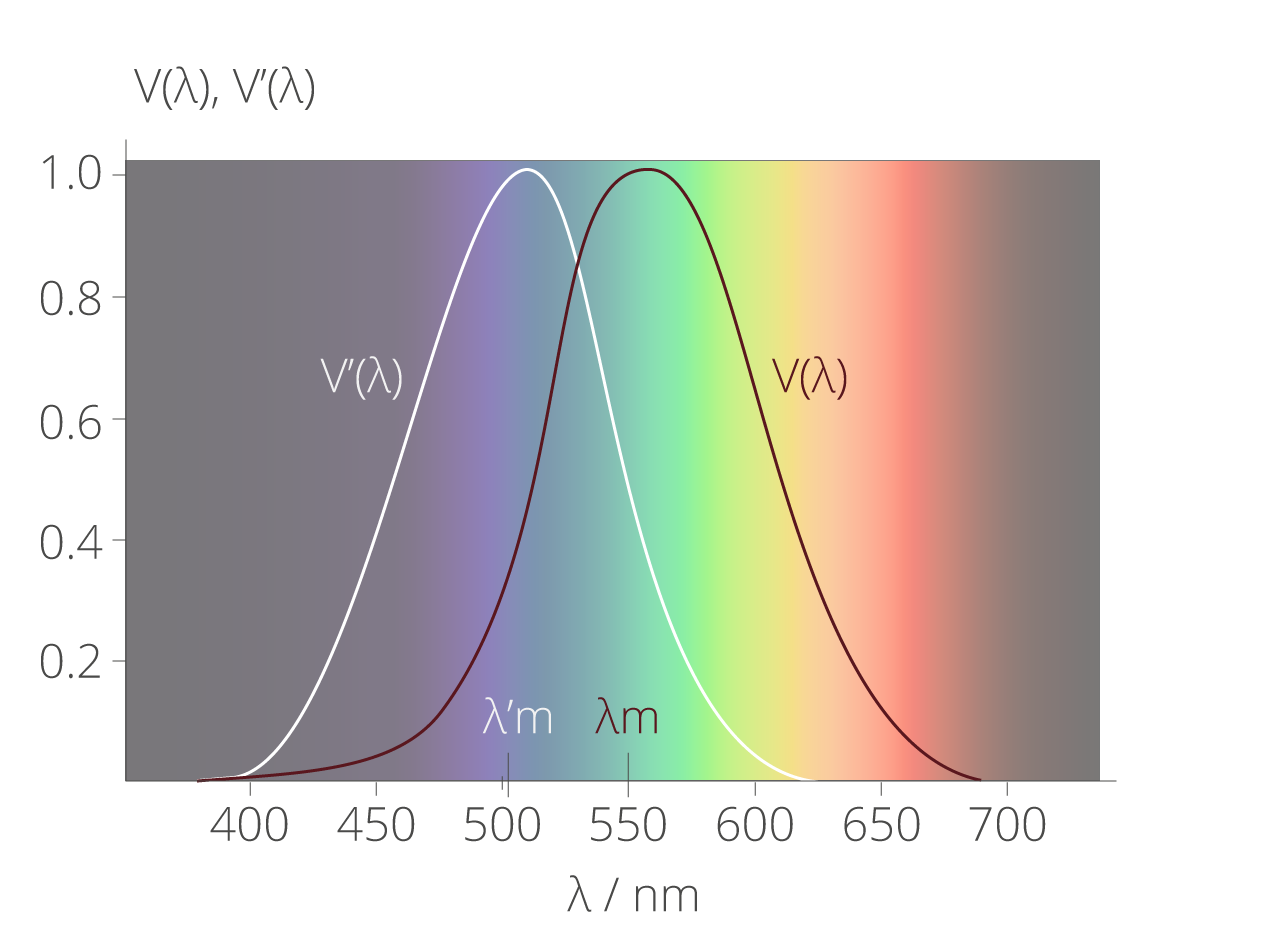
\includegraphics[width=0.7\textwidth]{bilder/augespek} 
% Bilddatei aus dem Unterverzeichnis bilder holen, skalieren auf 0.8*Satzspiegel
\caption {Die V($\lambda$)-Kurve zeigt, wie das Auge die verschiedenen Wellenlänge beim photopischen Sehen gewichtet. Die weiße Kurve (V'($\lambda$)) beschreibt, wie sich das Farbsehen beim Nachtsehen verschiebt. \protect\footnotemark}\label{b_augespek}
\end{figure}

\footnotetext{\url{https://www.gigahertz-optik.de/assets/Uploads/Abb.-II.13-neu-v03.png}}


Mit den Zapfen und Stäbchen kann ein Mensch bis zu 200 verschiedene Farbtöne wahrnehmen. Wenn man die verschiedenen möglichen Helligkeiten und Weißkombinationen dieser Farbtöne zusätzlich in Betracht zieht, kann man von ca. 20 Millionen unterschiedlichen Farben sprechen, die ein Mensch erkennen kann \footnote{\cite{unimann}}.
 
Um all diese Farben unterscheiden zu können gibt es nach Young und Helmholtz drei Rezeptortypen. Die \glqq Trichromatische Theorie\grqq\ besagt, dass es grüne, blaue und rote Zapfen gibt, die unterschiedlich empfindlich für die jeweiligen Spektralanteile des Lichtes sind. Aus diesen drei Farbinformation (RGB-Werte) entsteht dann im Gehirn eine Farbe. Auf diese Weise lassen sich aber nicht alle Phänomene der Farbwahrnehmung erklären. 1878 hat Hering eine andere Theorie entwickelt, wie Farben wahrgenommen werden und diese \glqq Gegenfarbentheorie\grqq\ genannt. Die Theorie besagt, dass es immer zwei Farben gibt, die sich gegensätzlich verhalten: rot und grün, blau und gelb und der unbunte Gegensatz schwarz (dunkel) und weiß (hell).\\ Nach ein paar Jahren der Uneinigkeit, welche der genannten Theorie denn nun korrekt ist, hat 1905 v. Kries mit seiner \glqq Zonentheorie\grqq\ herausgestellt, dass beide Theorien zugleich zutreffen. In der ersten Zone wird im Auge nach der \glqq Trichromatische Theorie\grqq\ eine Farbe als RGB-Stimulus wahrgenommen, dieser wird dann in der zweiten Zone nach der \glqq Gegenfarbentheorie\grqq\ im Gehirn mit den drei Farbgegensätzen ausgewertet \footnote{\cite[104]{hentschel}} (Abbildung \ref{b_zonen}).

 
\begin{figure}[H]     % h=here, t=top, b=bottom, p=page
\centering
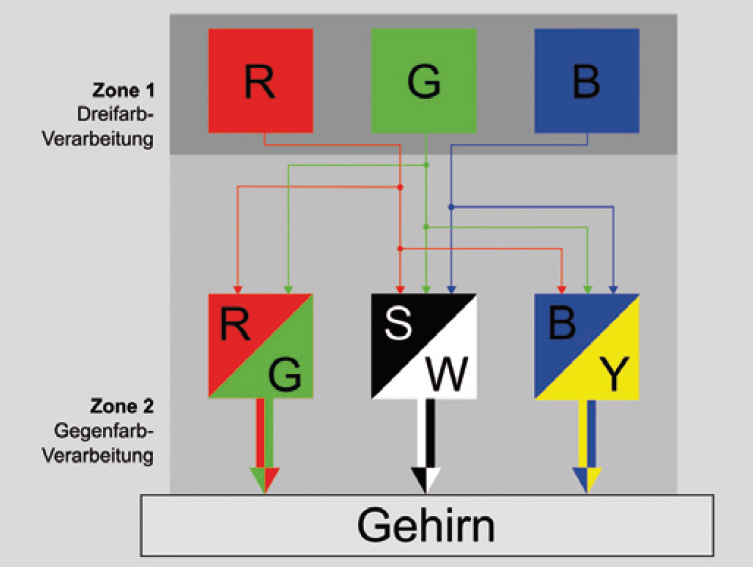
\includegraphics[width=0.7\textwidth]{bilder/zonen} 
% Bilddatei aus dem Unterverzeichnis bilder holen, skalieren auf 0.8*Satzspiegel
\caption {Darstellung der \glqq Zonentheorie\grqq\ von v. Kries \protect\footnotemark}\label{b_zonen}
\end{figure}
\footnotetext{\cite[153]{greule}}

%Überleitung schreiben

Bei der additiven Farbmischung werden die Spektralanteile verschiedener Farbtöne als Mischfarbe erkannt. Dies kann auf unterschiedliche Weisen passieren. Entweder treffen zwei verschiedene Spektralanteile auf den gleichen Punkt auf der Netzhaut und lösen so einen Farbreiz aus. Oder das Licht verschiedener Wellenlängen trifft auf unterschiedliche Teile der Netzhaut, die so dicht aneinander sind, dass das Auge daraus eine Farbe mischt (örtliche Nähe). Oder derselbe Punkt auf der Netzhaut wird von zwei verschiedenen Spektralanteilen mit einer Wechselfrequenz von $f\geq25Hz$ getroffen (zeitliche Nähe). Oder das Licht verschiedener Wellenlängen trifft auf unterschiedliche Teile der Netzhaut, die so dicht aneinander sind, dass das Auge daraus eine Farbe mischt.\\
Grundsätzlich werden bei jeder Art der additiven Farbmischung die Strahlungsleistungen der Spektralanteile $\Phi_{e\lambda,i}(\lambda)$ zusammenaddiert\footnote{\cite[83]{greule}}(Gleichung\ref{gl_farbe+}).

	\begin{equation}\label{gl_farbe+}
		\Phi_{e\lambda}(\lambda) = \Phi_{e\lambda,1}(\lambda) + \Phi_{e\lambda,2}(\lambda) + \Phi_{e\lambda,3}(\lambda)
	\end{equation}\\


1853 hat Grassmann zur additiven Farbmischung drei allgemein gültige Regeln aufgestellt \footnote{\cite[105]{hentschel}}: 
\newpage
\begin{enumerate}\setlength{\itemsep}{0ex}
\item Für das Ergebnis einer additiven Farbmischung ist nur das Aussehen, nicht die spektrale Zusammensetzung der Komponenten maßgebend.
\item Alle Farbmischungen verlaufen stetig.
\item Zum Festlegen einer Farbe sind drei Bestimmungsstücke notwendig und hinreichend.
\end{enumerate}

Die erste Regel beschreibt beispielweise das Verhalten einer Tomate unter gemischtem und ungemischtem magentafarbenen Licht. Wird die Tomate von einem magentanen Licht bestrahlt, dessen Spektrum nur Anteile im Magentabereich hat, so wird die Tomate weitesgehend unbunt erscheinen, weil diese alle spektralen Anteile des Lichts, außer den roten, absorbiert. Falls man aber rotes Licht mit blauem Licht mischt und so die selbe Lichtfarbe wie von dem reinen magentafarbigen Licht erzeugt, so erscheint die Tomate unter diesem Licht wiederum trotzdem rot, da die Rot-Anteile im Spektrum vorhanden sind. Man kann jedoch mit dem bloßen Auge diese beiden Farben nicht unterscheiden (metamere Farben), da der Mensch die spektrale Zusammensetzung von Licht nicht wahrnimmt. 

Die zweite Regel zeigt auf, dass bei der additiven Farbmischung die Farben stets ineinander übergehen und kein Sprung dabei entsteht, wenn zwei Farben zu einer Mischfarbe werden.

Die dritte Regel besagt, dass die additive Farbmischung beispielsweise über die Grundfarben Rot, Blau und Grün definiert werden kann. In der Abbildung   \ref{b_farben+} ist dargestellt wie aus den Grundfarben die Farben gemischt werden.

\begin{figure}[H]     % h=here, t=top, b=bottom, p=page
\centering
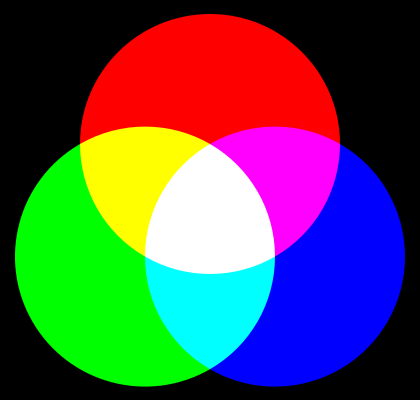
\includegraphics[width=0.5\textwidth]{bilder/farben+} 
% Bilddatei aus dem Unterverzeichnis bilder holen, skalieren auf 0.8*Satzspiegel
\caption {Die drei Grundfarben Rot, Grün und Blau der additiven Farbmischung ergeben zusammen weiß (unbunt).\protect\footnotemark}\label{b_farben+}
\end{figure}

\footnotetext{\url{https://upload.wikimedia.org/wikipedia/commons/thumb/e/e0/Synthese\%2B.svg/420px-Synthese\%2B.svg.png}}

Bei der subtraktiven Farbmischung geht es nicht um die Farbwahrnehmung des Auges, sondern um Licht im rein physikalischen Sinne. Ein subtraktives Farbgemisch entsteht, wenn die Transmissions- und Reflektionseigenschaften zweier Farben miteinander multipliziert werden\footnote{\cite[84]{greule}} (Gleichung \ref{gl_farbe-}).

\begin{equation}\label{gl_farbe-}
		T(\lambda) = T_{1}(\lambda) \cdot T_{2}(\lambda) \cdot T_{3}(\lambda)
	\end{equation}
Die Formel stellt ein Beispiel für das Produkt der Transmissionswerte dar.
Hierbei handelt es sich um ein wesentlich komplizierteren Prozess als bei der additiven Farbmischung. Da durch diese Multiplikation der Farben ein spektraler Anteil entfällt, spricht man von einer subtraktiven Farbmischung, obwohl das Produkt der Farbeigenschaften gebildet wird (Abbildung \ref{b_farben-}).

\begin{figure}[H]     % h=here, t=top, b=bottom, p=page
\centering
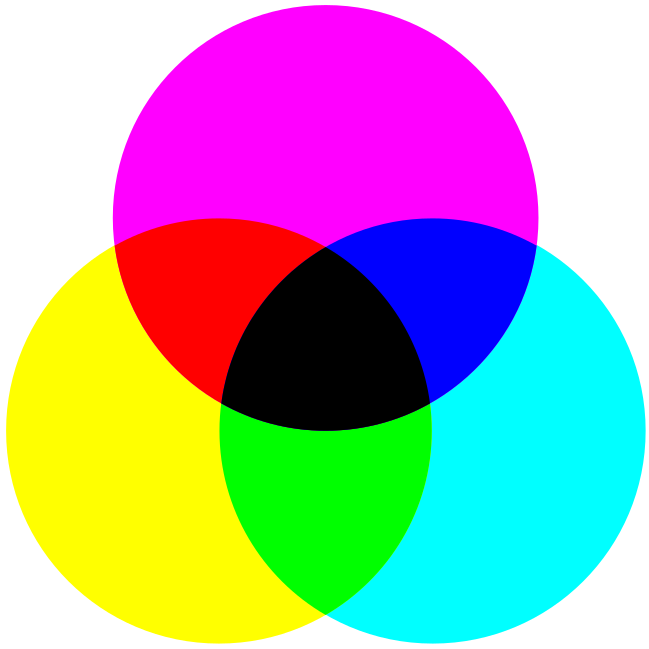
\includegraphics[width=0.5\textwidth]{bilder/farben-} 
% Bilddatei aus dem Unterverzeichnis bilder holen, skalieren auf 0.8*Satzspiegel
\caption {Die drei Grundfarben Cyan, Magenta und Gelb der subtraktiven Farbmischung ergeben zusammen schwarz (unbunt).\protect\footnotemark}\label{b_farben-}
\end{figure}


\footnotetext{\url{https://upload.wikimedia.org/wikipedia/commons/thumb/6/64/CMY_ideal_version_rotated.svg/649px-CMY_ideal_version_rotated.svg.png}}

Wenn man alle drei Grundfarben der subtraktiven Farbmischung mischt entsteht schwarz, weil dann alle Anteile im Licht abgezogen wurden.

%Überleitung zum RGB Farbraum

\section{Hauttöne}
 
\section{RGB Farbraum} \label{sec_rgb}
Durch die Festlegung verschiedener Farbräume hat die CIE die Farben von Licht immer besser einordnen und beschreiben können. Der große Vorteil bei diesen Farbräumen besteht darin, dass man durch eine lineare Transformation von einer Farbraumdarstellung in die nächste Wechseln kann und die spektrale Empfindlichkeitskurve mit transformiert wird. So wird sichergestellt, dass jede Farbe nach der natürlichen Wahrnehmung des Menschen gewertet wird.
Angefangen hat all dies mit dem RGB-Farbraum. Dieser Farbraum wird mit den drei Grundfarben der additiven Farbmischung, den Primärvalenzen Rot, Grün und Blau aufgespannt. Die Farben ergeben jeweils die Ecken und in der Mitte entsteht so der Weißpunkt des Farbraumes. Eine Farbe lässt sich dann über die Farbwertanteile r, g und b in diesem Farbraum orten\footnote{\cite[106]{hentschel}} (Gleichung \ref{gl_rgb1}).

\begin{equation}\label{gl_rgb1}
		r = \frac{R}{R+G+B},\quad g = \frac{G}{R+G+B},\quad b = \frac{B}{R+G+B}
\end{equation}
Der RGB-Farbraum ist so konstruiert, dass jede Kombination aus den drei Farbkoordinaten zusammen 1 ergibt. Es reichen also zwei Koordinaten aus, um den sogenannten Farbort bestimmen zu können, da sich die dritte Koordinate von selbst erschließt (Gleichung \ref{gl_rgb2}). 

\begin{equation}\label{gl_rgb2}
		b=1-r-g
\end{equation}

Man kann den RGB-Farbraum auch dreidimensional als Würfel aufspannen. Dort ist die Farbe schwarz der Ursprung und weiß die Kombination aus allen drei Farbvektoren (Abbildung \ref{b_rgb1}.

\begin{figure}[H]     % h=here, t=top, b=bottom, p=page
\centering
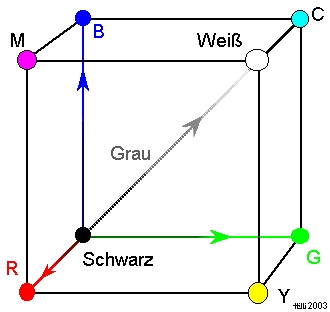
\includegraphics[width=0.5\textwidth]{bilder/rgb1} 
% Bilddatei aus dem Unterverzeichnis bilder holen, skalieren auf 0.8*Satzspiegel
\caption {Beim RGB-Würfel werden alle Primärvalenzen R,G, B als gleich lange Vektoren angenommen.\protect\footnotemark}\label{b_rgb1}
\end{figure}

 

\section{CIE-XYZ Farbraum} \label{sec_xyz}

Der RGB-Farbraum kann nicht alle Farben des sichtbaren Spektrum abbilden. Wright und Guild haben dazu Tests mit einem Monochromator gemacht. Ein Proband, der Farbflächen von $2^\circ$ Gesichtsfeldgröße sieht, sollte mit 700nm rot, 546nm grün und 435nm blau die gesehene Farbe nachmischen. Bei einer Referenzfarbe von 500nm blau-grün gab es keine Möglichkeit, diese Farbe mit den drei RGB-Farben zu mischen. Es musste sogar auf der Referenzfarbseite rot dazugemischt werden, damit man auf das Blau-Grün abgleichen konnte. Dies würde ein negativen Rot-Anteil im RGB-Farbraum bedeutet, den es so nicht geben kann. Daher hat die CIE 1931 ein virtuelles Primärvalenzssystem erarbeitet\footnote{\cite[77]{greule}}.\\
Im CIE-XYZ Farbraum gibt es die Primärvalenzen X, Y und Z, die aus einer linearen Transformation des RGB-Farbraum entstanden sind\footnote{\cite[76-77]{greule}} (Gleichungen  \ref{gl_xyz1} - 3.7).

\begin{eqnarray}\label{gl_xyz1}
		X = R_{x}\cdot R + G_{x}\cdot G + B_{x}\cdot B\\
		Y = R_{y}\cdot R + G_{y}\cdot G + B_{y}\cdot B\\
		Z = R_{z}\cdot R + G_{z}\cdot G + B_{z}\cdot B
\end{eqnarray}
Der Y-Wert entspricht dabei der Farbfunktion $y_{\lambda}$, die der $V(\lambda)$-Kurve (Abbildung \ref{b_augespek}) gleicht, und steht daher für die Helligkeit der Farbe. Dies ist eine Erweiterung zum RGB-Farbraum, in dem die Helligkeit nicht direkt mit einbezogen wurde. Der X-Wert zeigt den rot-grün-Anteil an und am Z-Wert lässt sich der Blau-Gelb-Anteil einer Farbe bestimmen\footnote{\cite[72]{mueller}}. 


Aus diesen Primärvarlenzen lassen sie dich Farbanteile ausrechnen, die auf der Farbtafel des CIE-XYZ Farbraums dargestellt werden (Gleichung \ref{gl_xyz2}). 
 

\begin{equation}\label{gl_xyz2}
		x = \frac{X}{X+Y+Z},\quad y = \frac{Y}{X+Y+Z},\quad z = 1-x-y
\end{equation}
Auch hier reichen zwei Normfarbwertanteile aus, um den Farbort (x,y) zu bestimmen. x steht für den Farbton und y für die Sättigung. Aus x und y kann jedoch kein Rückschluss auf die X, Y und Z Normalvalenzen gezogen werden und so ist zum Beispiel eine Bestimmung der Helligkeit (Y) aus dem Farbort nicht möglich\footnote{\cite[79]{greule}}.\\
Über die Grenzen des mit x und y aufgespannten Farbraums erstrecken sich von 380nm blau zu grün und gelb zu 780nm rot alle sichtbaren Farben des Spektrums. Die beiden Enden des Farbraumes sind auf der gegenüberliegenden Seite über die theoretische Purpur-Graden miteinander verbunden. Die Farben auf dieser Geraden werden vom menschlichen Auge magenta intertpretiert, gehören aber nicht mehr zum sichtbaren Wellenlängenbereich dazu\footnote{\cite[73]{mueller}}. Der Unbuntpunkt liegt bei $x=y=0,33$ (Abbildung \ref{b_xyz1}).

\begin{figure}[H]     % h=here, t=top, b=bottom, p=page
\centering
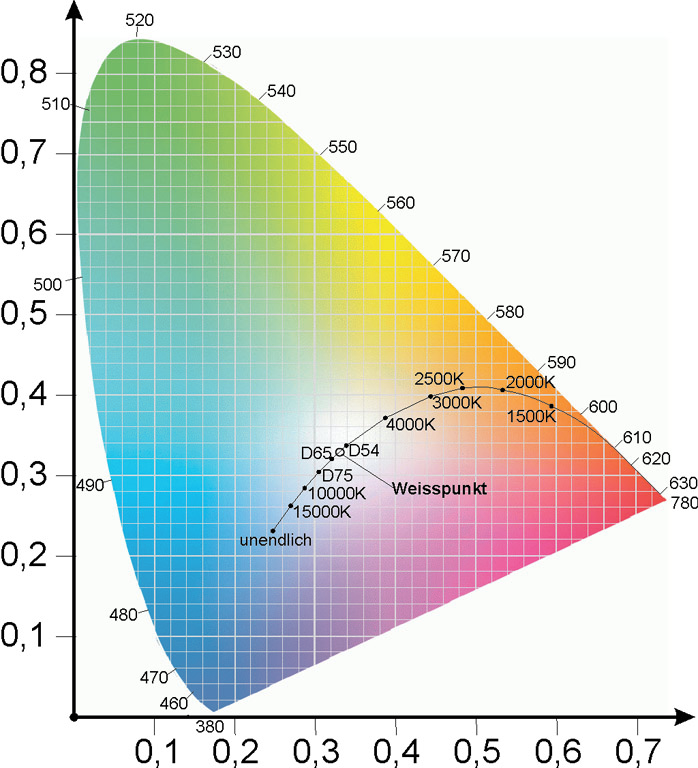
\includegraphics[width=0.8\textwidth]{bilder/xyz1} 
% Bilddatei aus dem Unterverzeichnis bilder holen, skalieren auf 0.8*Satzspiegel
\caption {Darstellung der CIE-XYZ Farbtafel eines 2$2^\circ$ Normalbeobachter. Diese Bezeichnung entstammt aus den Tests von Wright und Guild. \protect\footnotemark}\label{b_xyz1}
\end{figure}

\footnotetext{\url{https://www.production-partner.de/wp-content/uploads/2018/02/Farbdreieck.jpg}}

Im XYZ-Farbdiagramm ist der Plank'sche Kurvenverlauf eingezeichnet. Wenn ein Farbort auf diese Kurve trifft wird ihm die jeweilige Farbtemperatur zugeschrieben. Landet der Farbort in der Nähe dieser Kurve spricht man von einer korrelierten Farbtemperatur (CCT).  Es wurden so genannte \glqq Geraden ähnlichster Farbtemperatur\grqq\ bestimmt, die anzeigen welche korrelierten Farbtemperatur vom Farbort getroffen wird (Abbildung \ref{b_cct})    

\begin{figure}[H]     % h=here, t=top, b=bottom, p=page
\centering
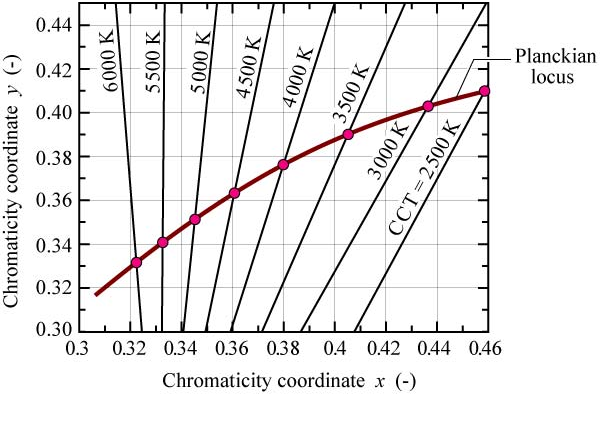
\includegraphics[width=0.8\textwidth]{bilder/cct} 
% Bilddatei aus dem Unterverzeichnis bilder holen, skalieren auf 0.8*Satzspiegel
\caption {Zoomansicht des XYZ-Farbraumes mit den \glqq Geraden ähnlichster Farbtemperatur\grqq\ \protect\footnotemark}\label{b_cct}
\end{figure}

\footnotetext{\url{http://www.light.fi/blog/wp-content/uploads/2016/04/xyChromaticity-diagram.png}}

Trifft eine Leuchte mit ihren x, y Normfarbwertanteilen auf einen Punkt über der Plank'schen Kurve, so erscheint der Weißton grünstichig, trifft sie unter die Kurve, dann wirkt das Weiß magentastichig. Ist der Farbort zu weit von der Plank'schen Kurve entfernt, kann keine Farbtemperatur bestimmt werden.\\

Wenn man zwei Farben im XYZ-Farbraum vergleichen will, ist vorsichtig geboten, da die Farben auf der Farbtafel nicht mit gleich großem Abstand dargestellt werden. Dies ist daran zu erkennen, dass die Farbabstände im roten (620nm - 770nm) und blauen (380nm - 470nm) Bereich sehr nahe beieinander liegen, wohingehen sich der grüne Bereich(500nm - 570nm) sich über einen großen Anteil des hufeisenförmigen Rand erstreckt. Farbkontraste verhalten sich also nicht wie mit dem Auge wahrgenommenen Farben. Mit diesem Phänomen hat sich MacAdam beschäftigt und so sind 1940 die \glqq MacAdam Ellipsen\grqq\ entstanden (Abbildung \ref{b_ellipsen}).

\begin{figure}[H]     % h=here, t=top, b=bottom, p=page
\centering
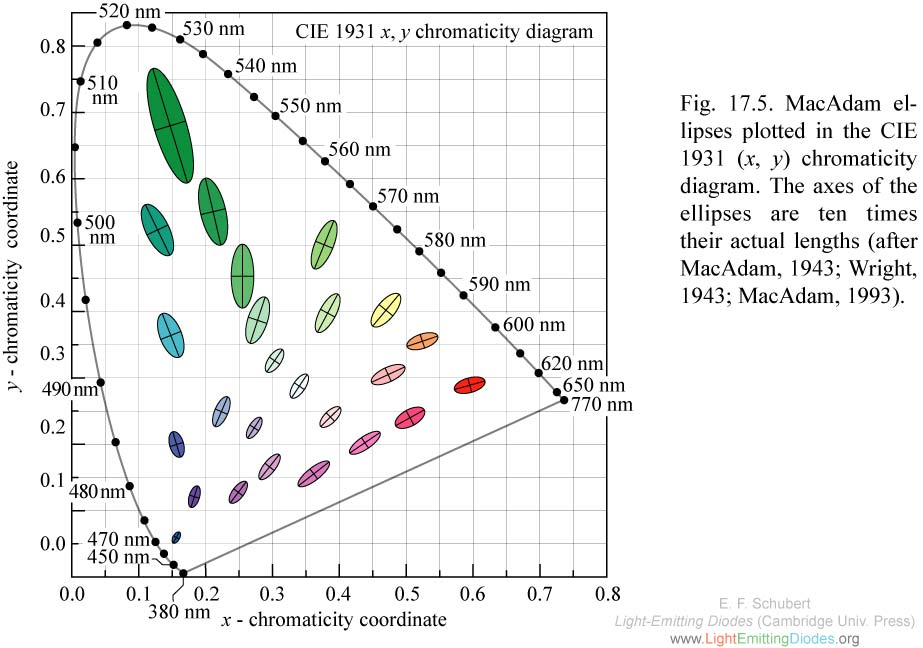
\includegraphics[width=1.0\textwidth]{bilder/ellipsen} 
% Bilddatei aus dem Unterverzeichnis bilder holen, skalieren auf 0.8*Satzspiegel
\caption {Abbildung der MacAdam Ellipsen im XYZ-Farbraum\protect\footnotemark}\label{b_ellipsen}
\end{figure}

\footnotetext{\url{https://ecse.rpi.edu/~schubert/Light-Emitting-Diodes-dot-org/chap17/F17-05\%20MacAdam\%20ellipses.jpg}}
Die MacAdam Ellipsen zeigen die Bereich an, in dem ein Normbalbeobachter zwei unterschiedliche Farborte dem selben Farbton zuordnen würde. Hätte der Farbraum annähernd gleiche Farbabstände, dann wären die Ellipsen kreisförmig.\\
Es wird also deutlich, dass der XYZ-Farbraum ein paar Schwächen aufweist. Das liegt daran, dass die X, Y und Z Primärvalenzen nur auf der additven Farbmischung beruhen. Die subtraktive Farbmischung, die ihr weiß aus 100\% Cyan, Magenta und Gelb mischt, ist in dieser Farbraumdarstellung nicht darstellbar (Farben  mit voller Sättigung liegen auf dem Kurvenrand). Außerdem hat MacAdam gezeigt, dass die Farbabstände nicht mit der realen Farbwahrnehmung zusammenhängt. So eignet sich der CIE-XYZ-Farbraum nur zur eindeutigen Bestimmung eines Farbreizes \footnote{\cite[79-80]{greule}}.


\section{CIE-unity chromity scale-Farbtafel (CIE-UCS)} \label{sec_ucs}
Damit die Farbabstände aus der Farbtafel besser mit der tatsächlichen Farbwahrnehmung übereinstimmt hat die CIE 1976 die UCS-Farbtafel definiert.

Für diese Farbtafel werden die x und y Normfarbwertanteile so transformiert, dass die Farbabstände vereinheitlicht sind (Gleichgung \ref{gl_ucs1}).

\begin{equation}\label{gl_ucs1}
		u' = \frac{4x}{-2x+12y+3} \quad v' = \frac{9y}{-2x+12y+3}
\end{equation}

Es wurden also die Farbbereiche aneinander angeglichen und die Farbtafel hat sich gedreht. Dadurch ähneln die Farbabständen den real empfunden Abständen schon deutlich besser als im XYZ-Farbraum. Durch die Transformation sind auch die MacAdam Ellipsen deutlich kreisförmiger geworden (Abbildung \ref{b_ucs}).  

\begin{figure}[H]     % h=here, t=top, b=bottom, p=page
\centering
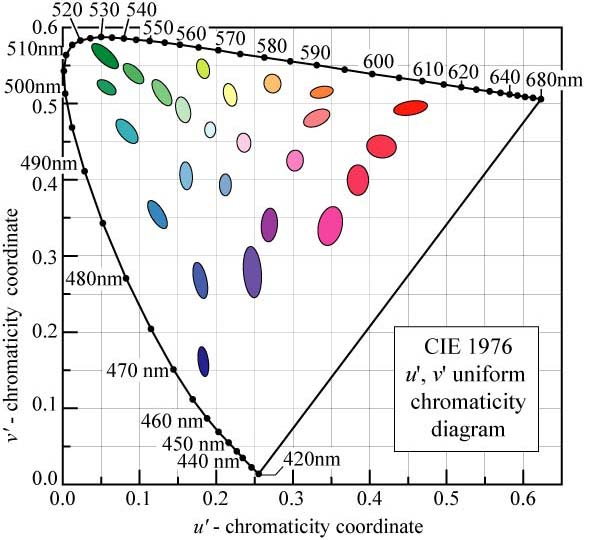
\includegraphics[width=0.8\textwidth]{bilder/ucs} 
% Bilddatei aus dem Unterverzeichnis bilder holen, skalieren auf 0.8*Satzspiegel
\caption {Abbildung der MacAdam Ellipsen auf der UCS-Farbtafel \protect\footnotemark}\label{b_ucs}
\end{figure}

\footnotetext{\url{https://www.fktg.org/sites/default/files/sauter_bild_02.jpg}}

Durch die CIE-UCS Farbtafel ist auch der $\Delta$u'v' entstanden. Dieser Wert ist wie beim TLCI (Kapitel \ref{sec_tlci}) ein Maß dafür, wie weit ein $u'_{i}$, $v'_{i}$ - Farbort mit korrelierter Farbtemperatur x von dem Plank'schen Kurvenzug bei Farbtemperatur x ($u'_{0}$, $v'_{0}$) entfernt ist\footnote{\cite[566]{jiyupe}} (Abbildung \ref{b_duv}).

\begin{figure}[H]     % h=here, t=top, b=bottom, p=page
\centering
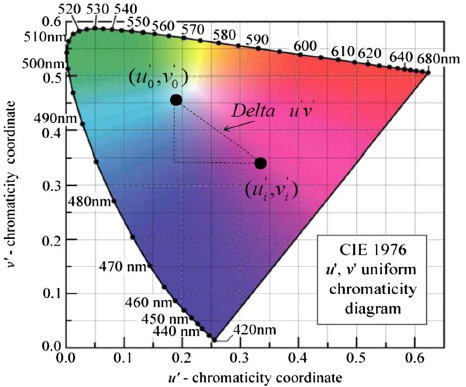
\includegraphics[width=0.8\textwidth]{bilder/duv1} 
% Bilddatei aus dem Unterverzeichnis bilder holen, skalieren auf 0.8*Satzspiegel
\caption {Darstellung des $\Delta$u'v' auf der UCS-Farbtafel}\label{b_duv}
\end{figure}


Anhand des Wertes ist erkennbar, ob das gemischte Weiß grünstichig mit $\Delta u'v' < 0$ oder magentastichtig mit $\Delta u'v' > 0$ ist (Gleichung \ref{gl_duv1}).

\begin{equation}\label{gl_duv1}
		\Delta u'v'=\sqrt{(du')^{2}+(dv')^{2}}=\sqrt{(u'_{i}-u'_{0})^{2}+(v'_{i}-v'_{0})^{2}}
\end{equation}

Dieser Wert wird zur Einschätzung der Weißlichtqualität in Kombination mit einem Farbwiedergabewert zur Rate gezogen und ist daher auch bei den \glqq Red Tail\grqq\ -Messung von größerer Bedeutung. Eine Abweichung von $\Delta u'v' < \pm 0.005$ ist für ein gutes weiß akzeptabel\footnote{\cite{ohno}}.\\

Auf der UCS-Farbtafel lassen sich nur Farben gleicher Helligkeit miteinander vergleichen. Um Farben verschiedener Helligkeiten vergleichen zu können hat die CIE noch weitere dreidimensionale Farbräume bestimmt, die für die Red-Tail-Untersuchungen, aber keine größere Rolle spielen.\newpage


\chapter{Lichtechnische Parameter}
Es gibt mehr als vierzig verschiedene Methoden, um die Farbwiedergabe einer Leuchte zu beurteilen. In diesem Kapitel sollen die in der Medien- und TV-Branche typischen Farbwiedergabeindices vorgestellt und deren Relevanz für die Messung mit dem \glqq Red Tail\grqq\  aufgezeigt werden.

\section{CIE: Color Rendering Index (CRI)} \label{sec_cri}

Da der Farbort allein keine eindeutige Aussage über die Zusammensetzung des Spektrums zulässt, wurde 1965 von der Commission Internationale de l'Eclairage ein Testverfahren entwickelt, mit dem man die Farbwiedergabe (Color Rendering Index) einer Leuchte bestimmen kann. Dafür hat man acht Referenzfarben festgelegt. Bei einer CRI-Messung überprüft man also, wie gut eine Lichtquelle diese Körperfarben wiedergeben kann. Es wird dabei zwischen einem schwarzen Strahler(< 5000K) und Tageslicht(> 5000K) differenziert. Die gemessenen Unterschiede zu den Referenzfarben werden mit Werten von 0 bis 100 gewichtet($R_{1}$-$R_{8}$), wobei ein Wert von 100 aussagt, dass die Farbe bestmöglich wiedergegeben wird. Zuerst werden die einzelnen Indexwerte $R_{i}$ aus den Farbdifferenzen $\Delta E_{i}$ berechnet (Gleichung \ref{gl_cri1})\footnote{\cite{davis_ohno}}.

	\begin{equation}\label{gl_cri1}
		R_{i} = 100 - 4,6 \cdot \Delta E_{i}
	\end{equation}
Diese acht Werte werden schließlich arithmetisch gemittelt und es ergibt sich der Gesamtwert $R_{a}$ (Gleichung \ref{gl_cri2})\footnote{\cite{production partner}}.
	\begin{equation}\label{gl_cri2}
		R_{a} =\frac{1}{8} \sum_{i=1}^{8} R_{i}
	\end{equation}
In der DIN 6169 werden zur besseren Beurteilung der Farbwiedergabe die $R_{a}$-Werte in verschiedene Stufen unterteilt (Tabelle \ref{t_cri}).

	\begin{table}[htp] 
		\rowcolors{1}{}{lgray} 
		\centering
		\begin{tabular}{rlcc}  % Spalten nach Ausrichtung: l, c, r, p{breite} 
		\toprule
		\multicolumn{3}{c}{\large\sffamily Stufen des CRI}\\ 							
		\midrule
		1A & $R_{a} \geq 90$ & sehr hohe Anforderung\\ 
		1B & 90 > $R_{a} \geq 80$ & sehr hohe Anforderung\\
		2A & 80 > $R_{a} \geq 70$ & hohe Anforderung\\
		2B & 70 > $R_{a} \geq 60$ & hohe Anforderung\\
		3 & 60 > $R_{a} \geq 40$ & mittlere Anforderung\\
		4 & 40 > $R_{a} \geq 20$ & geringe Anforderung\\
		\bottomrule
		\end{tabular}
		\caption{$R_{a}$ eingeteilt in verschiedene Stufen\protect\footnotemark}	
		\label{t_cri}
	\end{table}
	\footnotetext{\cite[111]{hentschel}}

Ein hoher $R_{a}$-Wert beschreibt aber nur bedingt die Farbwiedergabe einer Leuchte, da beispielsweise keine Angabe über die Sättigung der Farben gemacht wird. Außerdem sind die acht Referenzfarben nur Pastelltöne, weil der CRI damals für Glühlicht entwickelt wurde. Gesättigte Farben fließen nicht in die Bewertung mit ein.
Das wirkt sich auch auf die Vergleichbarkeit von Leuchten aus. Zwei Scheinwerfer mit dem selben $R_{a}$-Wert von 90 können sehr unterschiedliche Spektren haben und damit sehr unterschiedlich Farben darstellen, trotz gleichem Farbwiedergabeindex.
Außerdem kann man nur schwer eine Aussage darüber machen, ob sich eine Leuchte mit einem guten CRI für Personenbeleuchtung eignet, weil Rottöne und Hauttöne in diesem Bewertungsverfahren fehlen.\\\\
Leuchtstofflampen nutzten den CRI aus, indem durch gezielte schmalbandige Peaks im Spektrum die Referenzfarben getroffen werden. Auf diese Weise kann zwar ein hoher CRI-Werte erreicht werden, aber kein breitbandiges und ausgefülltes Lichtspektrum entstehen. Daher sah sich die CIE gezwungen den Farbwiedergabeindex zu erweitern. In dem neueren $R_{e}$-Wert gibt es nun auch gesättigte Farben und eine Hautfarbe wird miteinbezogen (Abb. \ref{b_cri}).

\begin{figure}[htp]     % h=here, t=top, b=bottom, p=page
\centering
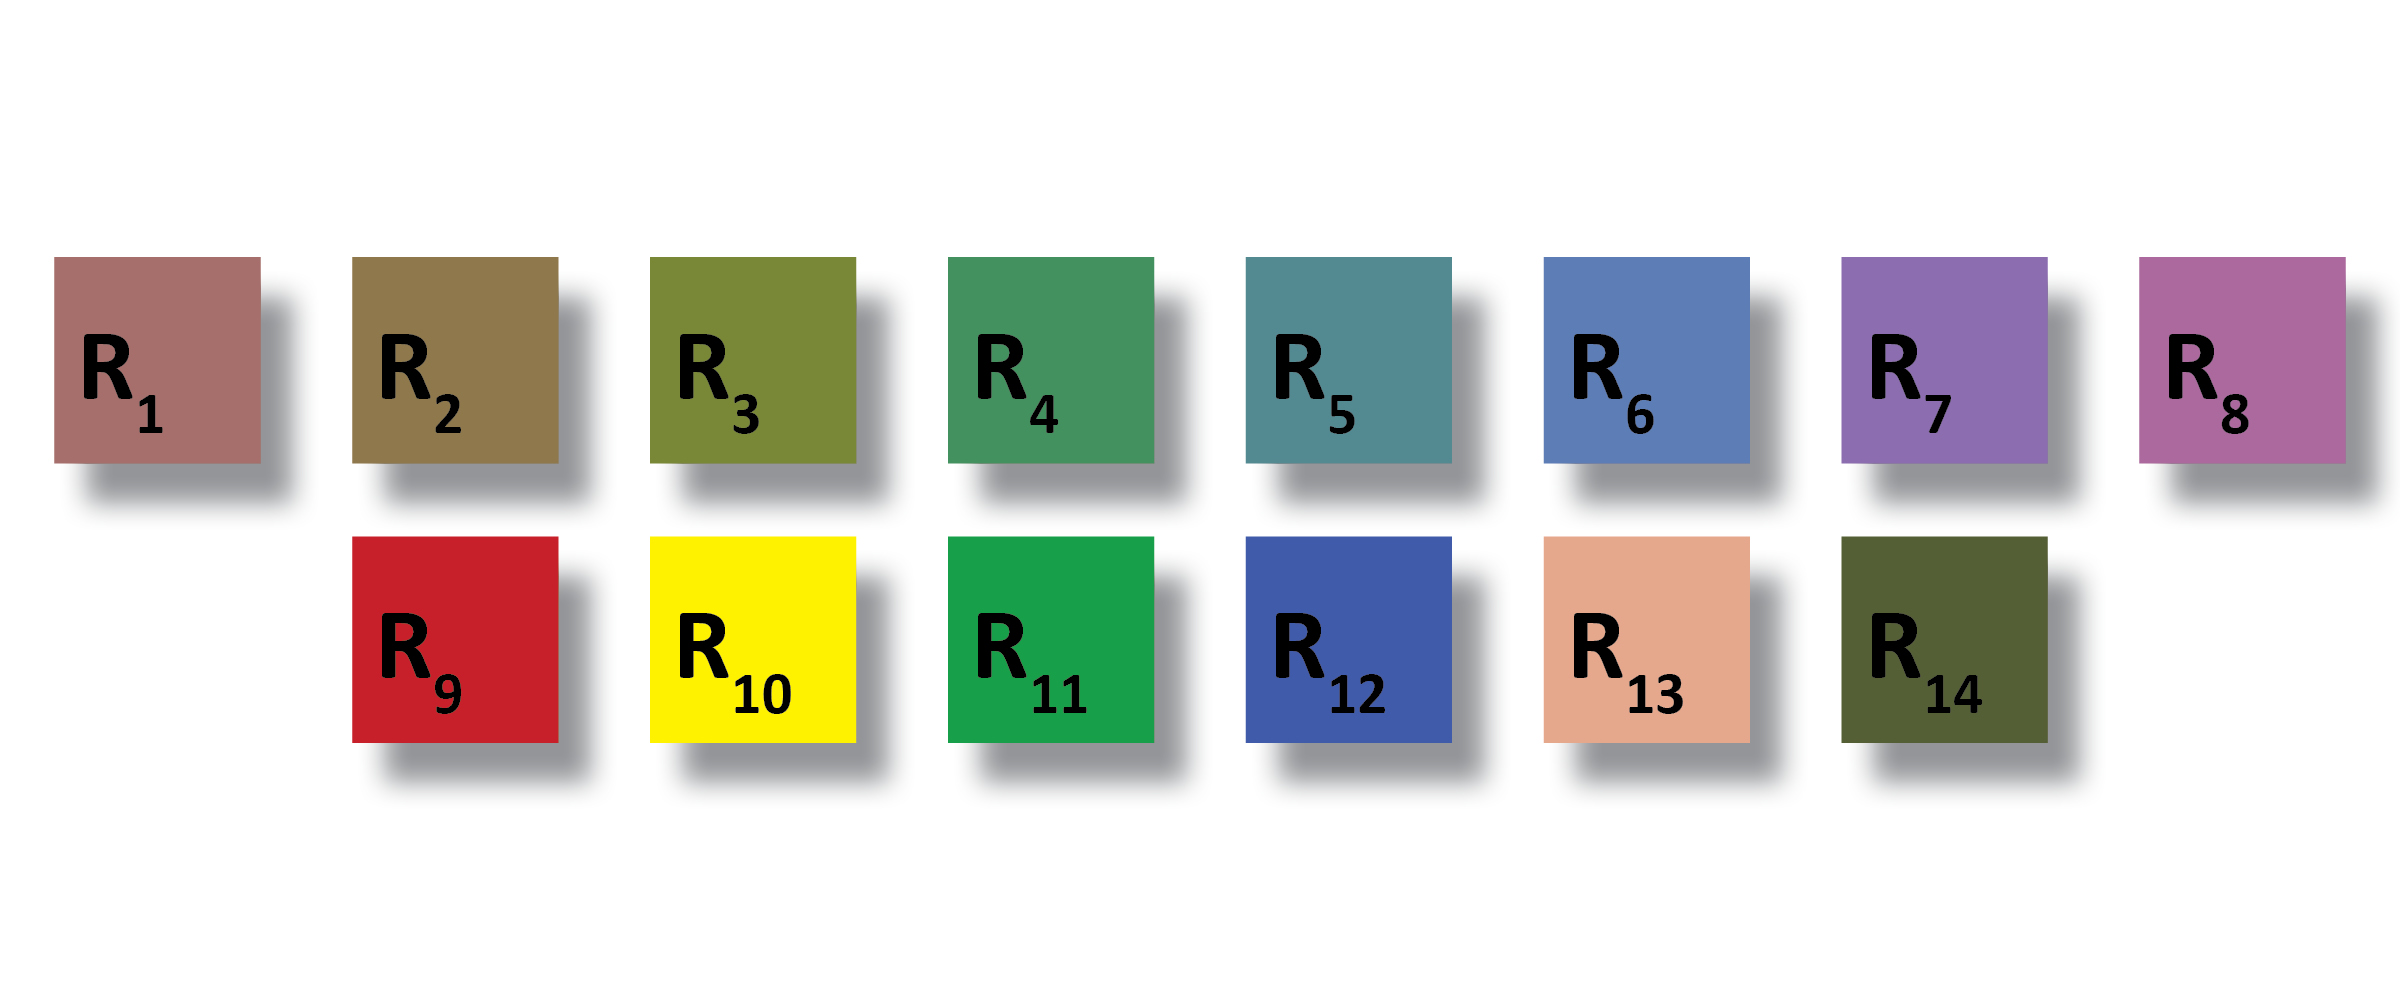
\includegraphics[width=0.8\textwidth]{bilder/cri} 
% Bilddatei aus dem Unterverzeichnis bilder holen, skalieren auf 0.8*Satzspiegel
\caption {Alle Referenzfarben des Farbwiedergabeindexes: $R_{1}$ Altrosa, $R_{2}$ Senfgelb, $R_{3}$ Gelbgrün, $R_{4}$ Hellgrün, $R_{5}$ Türkisblau, $R_{6}$ Himmelblau, $R_{7}$ Asterviolett, $R_{8}$ Fliederviolett, $R_{9}$ Rot gesättigt, $R_{10}$ Gelb gesättigt, $R_{11}$ Grün gesättigt, $R_{12}$ Blau gesättigt und $R_{13}$ Rosa (Hautfarbe), $R_{14}$ Blattgrün \protect\footnotemark}\label{b_cri}
\end{figure}

\footnotetext{\url{https://www.elementalled.com/wp/wp-content/uploads/2015/08/CRI_chart.jpg}}

Bei einer warmweißen LED konnte ein CRI von 82 gemessen werden (Abbildung \ref{b_cri2}). Der $R_{e}$-Wert ist naturgemäß schlechter als der $R_{a}$-Wert, aber auch dieser ist mit 77 noch akzeptabel, wenn man bedenkt, dass der $R_{9}$-Wert nur 15 Punkte erbringt. Diese Leuchte entspricht \glqq sehr hohen Anforderungen\grqq\ (Tabelle \ref{t_cri}) und ist damit nach Definition sehr gut in der Farbwiedergabe. Jedoch ist der $R_{9}$-Wert ein Hinweis darauf, dass man mit dieser Aussage vorsichtig sein sollte.

\begin{figure}[htp]     % h=here, t=top, b=bottom, p=page
\centering
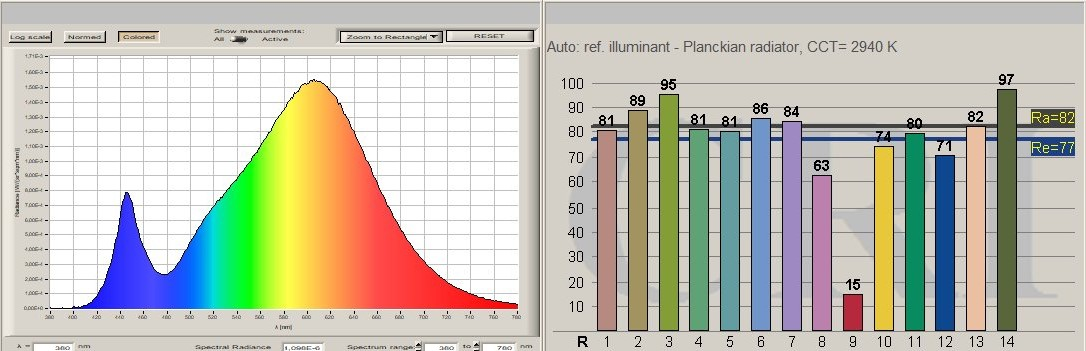
\includegraphics[width=1.0\textwidth]{bilder/cri2} 
% Bilddatei aus dem Unterverzeichnis bilder holen, skalieren auf 0.8*Satzspiegel
\caption {Messung einer warmweißen LED-Leuchte (Ausschnitt aus dem Demofile des Programmes \glqq LiVal\grqq\ von der Firma JETI): Links ist das Lichtspektrum der Leuchte dargestellt, rechts die gemessenen CRI-Werte  \protect\footnotemark}\label{b_cri2}
\end{figure}

Daher ist auch mit einem einzigen Rot- und Hautton der CRI zu wenig ausschlaggebend, um damit eine Leuchte für Personenbeleuchtung zu bewerten (Kap. \ref{sec_auge}). Zusätzlich entsteht bei LED-Leuchtmitteln ein ähnliches Problem, wie bei den Leuchstoffröhren. Man kann das Spektrum mit den Peaks gut auf die Referenzfarben ausrichten, ohne das Gesamte Spektrum abdecken zu müssen. Gerade bei LED-Leuchten kann dieses Verhalten des CRI ausgenutzt werden, um kritische Bereiche zu verschleiern. Zusätzlich wird dies durch die arithmetische Mittlung der Referenzfarbwerte begünstigt. Ein, zwei schlechtere Werte mindern den $R_{a}$-Wert nicht beträchtlich. Beispielsweise wird bei Weißen-LEDs der fehlende Rotanteil nur am niedrigen $R_{9}$-Wert sichtbar, aber im CRI-Wert sind diese Schwächen einer LED-Leuchte kaum erkennbar \footnote{\cite{davis_ohno}}. Der CRI kann daher eher als richtungsweisend betrachtet werden: Eine Leuchte mit guter Farbwiedergabe wird auch immer einen guten CRI-Wert haben. Zum Vergleich für Leuchten eignen sich andere Farbwiedergabewerte heutzutage besser \footnote{\cite{production partner}}.\\\\
Aus diesen Gründen und der Erkenntnis der CIE, \emph{\glqq dass die CRI-Methode generell nicht anwendbar ist, um eine Anzahl von Lichtquellen gemäß ihrer Farbwiedergabe einzuordnen, wenn weiße LEDs darunter sind\grqq}\footnote{\citep[VI]{CIE}}, wird sich diese Arbeit hauptsächlich auf andere Farbwiedergabewerte konzentrieren, den CRI aber mit aufführen, weil dieser in der Scheinwerfer- und Fernsehbranche (noch) einen hohen Stellenwert inne hat.

\section{NIST: Color Quality Scale (CQS)} \label{sec_cqs}

Der Color Quality Scale, der von dem National Institute of Standards and Technology (NIST) erarbeitet wurde, orientiert sich an der Grundidee des CRI und versucht dessen Probleme anzugehen und ihn zu ersetzen. So gibt es fünfzehn voll saturierte Referenzfarben, die auch auf LED-Leuchten anwendbar sind. Über Skaleneffekte soll der CQS auch indirekt eine Aussage über die Farbwiedergabe von Pastelltönen ermöglichen (Abb. \ref{b_cqs1}). 

\begin{figure}[htp]     % h=here, t=top, b=bottom, p=page
\centering

\includegraphics[width=0.8\textwidth]{bilder/cqs} 
% Bilddatei aus dem Unterverzeichnis bilder holen, skalieren auf 0.8*Satzspiegel
\caption {Alle Referenzfarben des CQS mit voller Sättigung\protect\footnotemark}\label{b_cqs1}
\end{figure}

\footnotetext{\url{https://www.lemoledlight.com/wp-content/uploads/2016/04/LED-Lighting-CRI-5.jpg}}
Bei dem Farbvergleich des CRI wurden weniger Punkte für eine Farbe vergeben, wenn diese übersättigt wurde, also die Leuchte eine höhere Farbigkeit hatte als das Referenzlicht des CRI. Wenn beispielsweise eine Oberfläche eines Objekts beleuchtet wird, kann eine übersättigte Farbe jedoch hilfreich sein und ist daher nicht pauschal negativ einzuordnen. Deswegen wertet der CQS eine Übersättigung der Farbe nicht, nur eine Abweichung von Farbton oder Helligkeit wird bestraft. Außerdem errechnet sich der CQS aus dem quadratischen Mittel (root-means-square) der einzelnen Farben und es ist deutlicher erkennbarer, wenn einzelne Farbe schlechte Werte erzielen (Gleichung \ref{gl_cqs1})\footnote{\cite{davis_ohno}}.

\begin{equation}\label{gl_cqs1}
		\Delta E_{rms} = \sqrt{\frac{1}{15} \sum_{i=1}^{15} \Delta E_{i} ^{2}} 
\end{equation}

Aus diesem Farbdifferenzwert wird ähnlich wie beim CRI (Gleichung \ref{gl_cri1}) ein Farbwiedergabewerte errechnet (Gleichung \ref{gl_cqs2}).

\begin{equation}\label{gl_cqs2}
		Q_{f,rms} = 100 - 3,0305 \cdot \Delta E_{rms} 
\end{equation}

Schließlich wird der CQS auf Werte von 0 bis 100 skaliert. Dadurch entfallen beim CQS negative Farbwerte, die beim CRI sehr schwierig zu interpretieren sind (Gleichung \ref{gl_cqs3}). 

\begin{equation}\label{gl_cqs3}
		Q_{f} = 10 \ln(e^{\frac{Q_{f,rms}}{10}}+1) 
\end{equation}\\

Der CQS wird mit seinen fünfzehn Referenzfarborten (abhängig von der Farbtemperatur) im CIELAB-Farbraum eingezeichnet. Da die Abstände von Farborten in diesem Farbraum in etwa wahrgenommenen Farbunterschieden entsprechen (Kap. \ref{sec_lab}), kann man gut erkennen, wie stark sich die Farbwiedergabe einer Leuchte den Referenzwerten ähneln(Abb. \ref{b_cqs2a} und \ref{b_cqs2b}).\\

\begin{figure}[htp]     % h=here, t=top, b=bottom, p=page
\centering
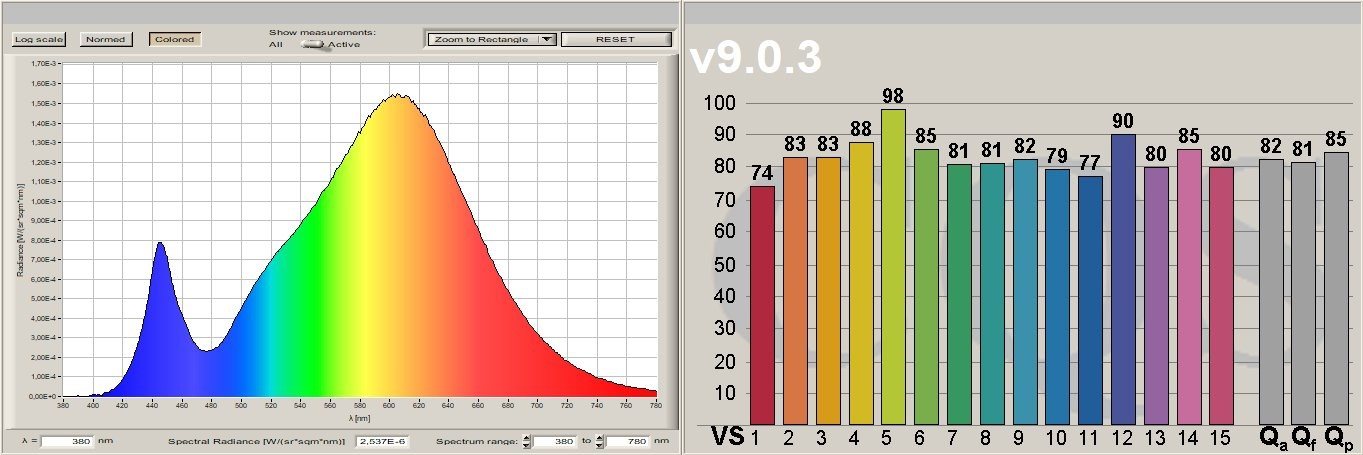
\includegraphics[width=0.9\textwidth]{bilder/cqs2a} 
% Bilddatei aus dem Unterverzeichnis bilder holen, skalieren auf 0.8*Satzspiegel
\caption {Ausschnitt aus dem Programm \glqq LiVal\grqq\ von der Firma JETI: Demo Spektrum einer warmweißen LED (2942K) mit $Q_{f} = 81$}\label{b_cqs2a}
\end{figure}

\begin{figure}[htp]     % h=here, t=top, b=bottom, p=page
\centering
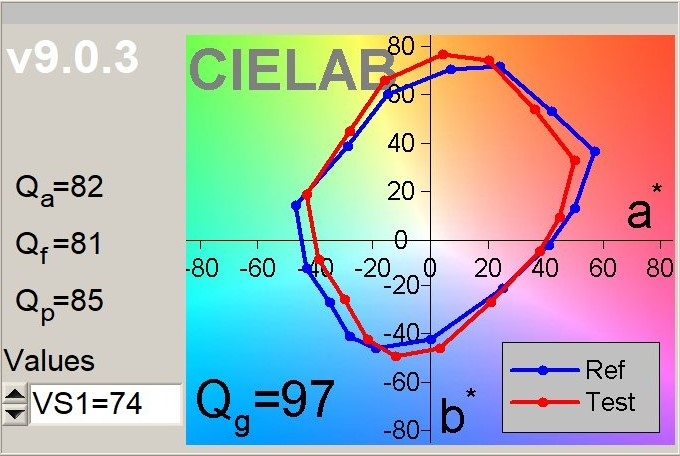
\includegraphics[width=0.7\textwidth]{bilder/cqs2b} 
% Bilddatei aus dem Unterverzeichnis bilder holen, skalieren auf 0.8*Satzspiegel
\caption {Ausschnitt aus dem Programm \glqq LiVal\grqq\ von der Firma JETI: Die fünfzehn Referenzfarben(blau) im CIELAB-Farbraum im Vergleich zu den gemessenen Werten (rot)}\label{b_cqs2b}
\end{figure}

Auf die in den Abbildung \ref{b_cqs2a} und \ref{b_cqs2b} erwähnten Werte $Q_{a}$ (optimierter CQS-Wert für kaum übersättigte Farben), $Q_{p}$ (optimierter CQS-Wert für viele übersättigte Farben) und $Q_{g}$(optimierter CQS-Wert im Zusammenhang mit dem Gamut Area Index) wird in dieser Arbeit nicht weiter eingegangen, weil sie über den Rahmen dieser Bachelorarbeit hinaus gehen\footnote{\cite[60-62]{khanh}}. \\
Da der CQS ähnlich wenige Referenzfarben nutzt wie der CRI, und keine besondere Aussage über die Farbwiedergabe von Hauttönen im TV-Bereich liefert, wird bei den Messungen dieser Arbeit das Hauptaugenmerk nicht auf dem CQS liegen. Der CQS eignet sich besser zur Einschätzung der Farbwiedergabe ohne Bezug zu einer TV-Kamera. 


\newpage 
\section{EBU: Television Lighting Consistency Index (TLCI)} \label{sec_tlci}
Der CRI-Wert einer Leuchte ist im Fernsehbereich kaum aussagekräftig, weil kein Bezug zur Videokamera besteht und die Farbwiedergabe von menschlichen Hauttöne kaum gemessen wird. Daher hat die European Broadcast Union (EBU) 2012 einen neuen Farbewiedergabe bestimmt, der auf den Film- und Fernsehbereich zugeschnitten ist, den Television Lighting Consistency Index.  
Wie eine Messung des TLCI vonstattengeht ist in diesem Blockschaltbild der EBU verdeutlicht (\ref{b_tlci1}):

\begin{figure}[htp]     % h=here, t=top, b=bottom, p=page
\centering
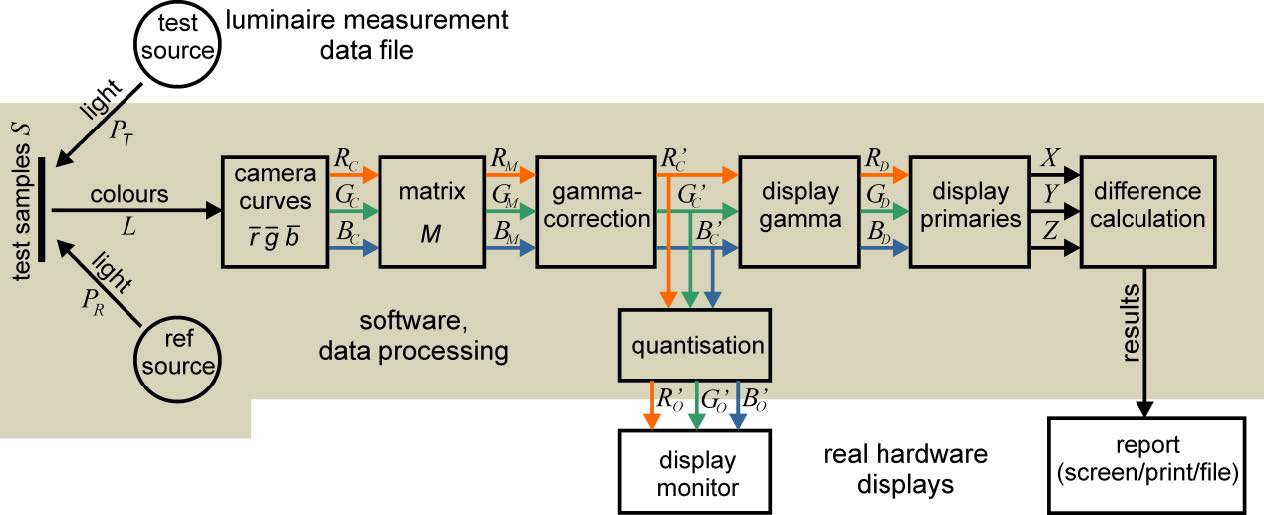
\includegraphics[width=1.0\textwidth]{bilder/tlci1} 
% Bilddatei aus dem Unterverzeichnis bilder holen, skalieren auf 0.8*Satzspiegel
\caption {Blockschaltbild einer TLCI-Wertbestimmung \protect\footnotemark}\label{b_tlci1}
\end{figure}
\footnotetext{\citep[15]{roberts}}
Die von der Kamera gefilmten Farben werden dann in einem Datenfile gespeichert. Die Daten werden analysiert, um die Farbtemperatur zu bestimmen und so die Referenzdaten zu erstellen.

Zur Ermittlung des TLCI wird eine Testtafel mit 24 Farben von einer \glqq Standartkamera\grqq\ gefilmt. Diese Tafel wird von der zu testenden Leuchte bestrahlt. Die Kamera ist an einen \glqq Standartbildschirm\grqq\ angeschlossen, auf dem die TLCI-Merssergebnisse angezeigt werden.
Im ersten Schritt gewichtet die Kamera die reflektierten Farben mit ihren $\bar{r}$-, $\bar{g}$- und $\bar{b}$-Kamerakurven und die Farbtemperatur wird bestimmt. Die so entstandenen $R_{C}$, $G_{C}$ und $B_{C}$-Werte werden dann im zweiten Schritt farblich abgeglichen ($R_{Cb}$, $G_{Cb}$ und $B_{Cb}$) und mit einer linearen Matrix M bewertet, um die Werte des RGB-Signals zu erhalten .
\begin{equation}\label{gl_tlci1}
\begin{bmatrix} R \\ G \\ B \end{bmatrix}= 
\begin{bmatrix} 1,182 & -0,209 & 0,027 \\ 0,107 & 0,890 & 0,003 \\ 0,004 & -0,134 & 1,094 \end{bmatrix}
\begin{bmatrix} R_{Cb} \\ G_{Cb} \\ B_{Cb} \end{bmatrix}
\end{equation}\\
Ein Weißabgleich wird vorgenommen und die RGB-Werte werden in einer zweiten Matrix verrechnet, damit die Sättigungswerte der Farben stimmen (Empfehlung der EBU: 90 \% Sättigung). Im nächsten Schritt werden die $R_{M}$, $G_{M}$ und $B_{M}$-Werte der einzelnen Farben von der Gammakurve der Kamera vorverzerrt.
Beim Bildschirm angekommen werden die R'G'B'-Werte der Farben mit der Gammakurve des Bildschirm wieder entzerrt (Empfehlung der EBU: $\gamma$ = 2,4). Für die 24 Farben werden dann im vorletzten Schritt mit der XYZ()-Matrix  die Farbkoordinaten X,Y und Z für den Bildschirm errechnet. Schließlich wird mit den Referenzenfarbwerten der selben Farbtemperatur die Farbunterschiede ermittelt (Gleichung \ref{gl_tlci1}).
\begin{equation}\label{gl_tlci1}
		\Delta E_{a} ^{*} = \left( {\sum_{i=1}^{18}(\Delta E_{i} ^{*})^{4}}  \right)^{\frac{1}{4}} 
\end{equation}
Das Ergebnis wird als TLCI-Wert ausgegeben. Für optimale Werte wird mit $k = 3,16$ (eine Tageslichtleuchtstoffröhre erreicht dabei den TLCI-Wert 50) und $p = 4$ (für ein balanciertes Verhältnis zwischen hohen und niedrigen Werten) gerechnet\footnote{\cite[16-22]{roberts}} (Gleichung \ref{gl_tlci2}).

\begin{equation}\label{gl_tlci2}
		Q = \frac{100}{1+(\frac{\Delta E^{*}}{k})^{p}}
\end{equation}

Der TLCI lässt wie der CQS keine negativen Ergebnisse zu (Kapitel \ref{sec_cqs}) und die Werte von 0-100 sind für den Coloristen in der Nachbearbeitung des Videomaterials wie folgt zu deuten(Tabelle \ref{t_tlci}):

	\begin{table}[htp] 
		\rowcolors{1}{}{lgray} 
		\centering
		\begin{tabular}{rlcc}  % Spalten nach Ausrichtung: l, c, r, p{breite} 
		\toprule
		\multicolumn{2}{c}{\large\sffamily Abstufungen des TLCI}\\ 							
		\midrule
		$100 \geq  Q_{a} \geq 85$  & Farben korrigierbar bzw. nicht notwendig\\ 
		$85 > Q_{a} \geq 75$ & nach Korrektur noch akzeptabel\\
		$75 > Q_{a} \geq 50$ & Aufbereitung sehr zeitaufwendig\\
		$50 > Q_{a} \geq 25$ & nicht mehr zu retten - verbesserbar\\
		$25 > Q_{a} \geq 0$ & ist und bleibt nicht akzeptierbar\\
		\bottomrule
		\end{tabular}
		\caption{$Q_{a}$ eingeteilt in verschiedene Stufen\protect\footnotemark}	
		\label{t_tlci}
	\end{table}
	\footnotetext{\cite{production partner}}
Anhand der Tabelle ist eine Art Kostenvergleich möglich, in dem die Farbwiedergabequalität einer Leuchte gegen den Nachbearbeitungsaufwand des Coloristen gegengerechnet werden kann. Der TLCI gibt sogar eine Empfehlung ab, an welchen Paramtern der Colorist Verbesserungen vornehmen muss (Abbildung \ref{b_tlci2}).\newpage 

Die Messung des TLCI-Werts ergibt ein Ergebnisprotokoll, bestehend aus drei Abschnitten: eine Farbtafel mit den 24 Farbfeldern, eine Empfehlung für den Coloristen zur nachträglichen Bildbearbeitung und ein Vergleich von Referenz- und Testspektrum (Abbildung \ref{b_tlci2}):\\ 

\begin{figure}[htp]     % h=here, t=top, b=bottom, p=page
\centering
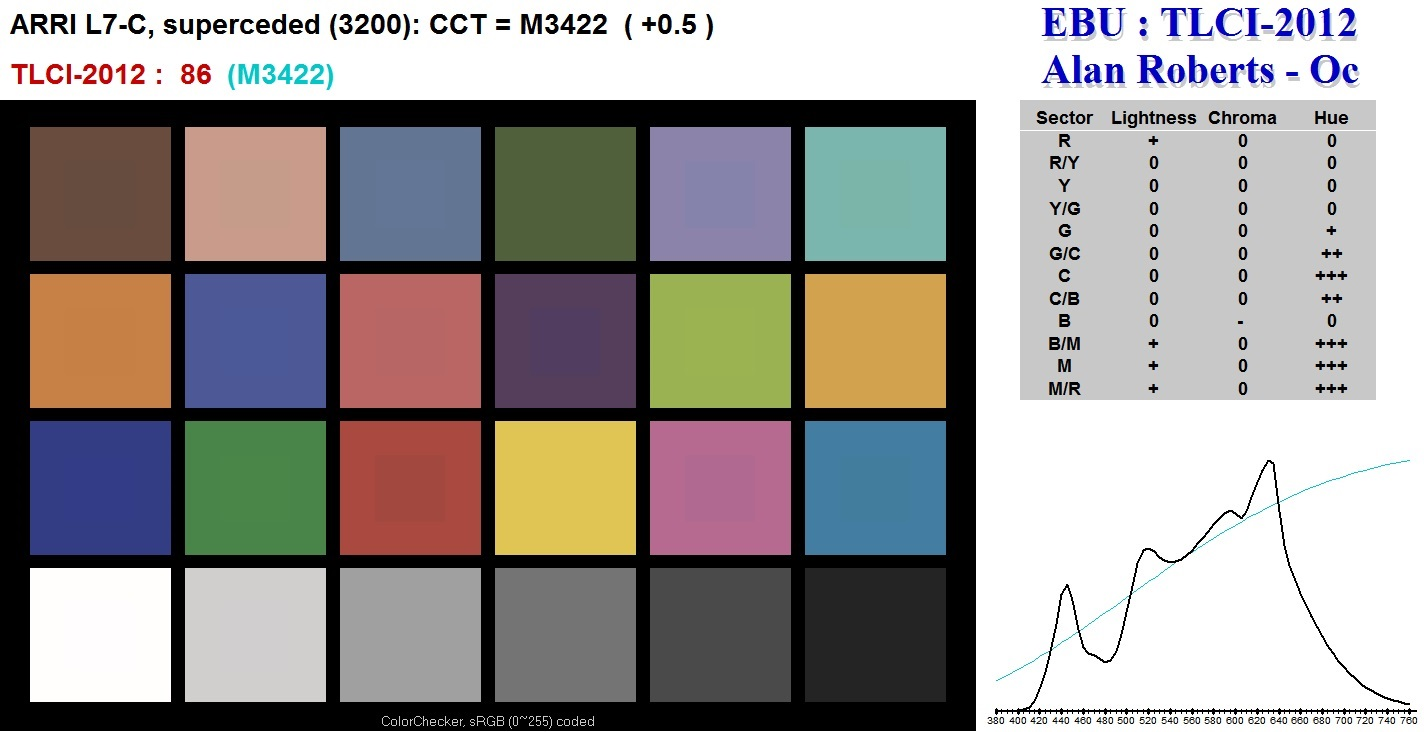
\includegraphics[width=1.0\textwidth]{bilder/tlci2} 
% Bilddatei aus dem Unterverzeichnis bilder holen, skalieren auf 0.8*Satzspiegel
\caption {TLCI-Ergebnisprotokoll eines Arri L7-C LED Fresnelscheinwerfers\protect\footnotemark}\label{b_tlci2}
\end{figure}
\footnotetext{\url{https://tech.ebu.ch/tlci-2012}}
Oben links ist der Name der Leuchte angegeben, die gemessene korrelierte Farbtemperatur (CCT) und die Abweichung vom Plank'schen Kurvenzug (\ref{sec_spektrum}) mit einer Gewichtung von 0.0054 (Empfehlung EBU). Ist der Abweichungswert kleiner als -1 wird die Zahl in magenta dargestellt (magentastichtiges weiß), ist sie größer als +1, in grün (grünstichiges weiß). Im Beispiel ist die Zahl daher schwarz. Eine Zeile darunter steht der gemessene TLCI-Wert. Der Arri L7-C ist mit $Q_{a}=86$ in die beste Farbwiedergabekategorie einzuordnen (Tabelle \ref{t_tlci}).\\
Oben rechts ist eine Tabelle mit Korrekturwerten für den Coloristen angegeben. Für 12 verschiedene Farbtöne wird jeweils ein Verbesserungsvorschlag für die Helligkeit, die Sättigung und die Farbtonabweichung angegeben. Da es nicht möglich ist, die Abweichung der Werte mit exakten Zahlen zu definieren, werden mit \glqq +\grqq\ , \glqq 0\grqq\ und \glqq -\grqq\ die verschiedenen Korrekturrichtungen aufgezeigt. Eine \glqq 0\grqq\ zeigt an, dass der Fehler zu klein ist, um ihn zu korrigieren. Die Anzahl der \glqq +\grqq\ und \glqq -\grqq\ wiederum ist ein Hinweis darauf, wie viel Aufwand der Colorist für die Anpassung benötigt. Der Arri L7-C hat beispielsweise Bedarf es vorallem im Bereich des Cyan, Blau/Magenta, Magenta und Magenta/Rot in der Farbtonabweichung einer Aufbesserung. Auch im Green/Cyan- und Cyan/Blau-Bereich sollte der Farbton angepasst werden. Die restlichen Verbesserungsvorschläge bei Helligkeit und Sättigung sollte der Colorist zügig bewältigen können.\\
Links unten ist eine Farbtafel mit den 24 Farben des TLCI sichtbar. Im großen Farbfeld ist die Farbe zusehen, wie das Licht des Arri L7-C diese Farbe wiedergibt. In der Mitte jeder Farbtafel ist ein kleineres Viereck, in dem die Referenzfarbe gezeigt wird. Je deutlicher also das Referenzviereck in dem Farbfeld zu sehen ist, desto schlechter ist die Farbwiedergabe der Testleuchte. Im Beispiel  ist im roten Farbfeld zu erkennen, dass der Arri L7-C diese Farbe nicht so gut wiedergibt wie andere Farben.\\ 
Rechts unten ist auf dem TLCI-Ergebnisprotokoll das Referenzspektrum von 380nm bis 740nm Wellenlänge abgebildet (schwarz) und dazu wird das geteste Spektrum geplotet (cyan). In dieser Ansicht kann man gut erkennen, inwieweit das Licht des Arri L7-C das Referenzspektrum abdeckt \footnote{\cite[15]{roberts}}.\\

Der TLCI sieht die Farben wie eine Kamera und zieht sogar zwei Hauttöne mit in Betracht. Daher eignet sich dieser Farbwiedergabewert sehr gut für die Messung der Auswirkung eines Red Tail.  



\section{IES Method for Evaluating Light Source Color Rendition (TM-30-15)} \label{sec_tm30}

Auch der TM-30 wurde 2015 von der \glqq Illuminating Engineering Society\grqq\ (IES) ausgearbeitet um eine Alternative zum CRI zu finden. Wie beim CRI werden ebenso bei der Messung des TM-30 Farbunterschiede zwischen einer Testleuchte und Referenzwerten der selben korrelierten Farbtemperatur aufgezeigt. Der TM-30 differenziert ähnlich, ob es sich bei der Testleuchte um einen Plank'schen Strahler  oder einem Tageslicht handelt. Zwischen einer CCT von 4500K und 5500K wird die Referenz proportional überblendet, um so zu verhindern, dass es bei 5000K einen \glqq Sprung\grqq\ gibt. Bei dem CRI konnte es nämlich passieren, dass eine Leuchte 2 unterschiedliche Referenzen bekam, je nach dem ob diese knapp über oder unter 5000K bei der Messung lag. 
Die 99 Referenzfarben (Color Evaluation Sample) wurden aus einem Pool von 105.000 Farbtönen realer Objekte statistisch ermittelt (Abbildung \ref{b_tm301}). Damit alle Farbtöne gleichmäßig abgedeckt werden, wurde der CAM02-UCS-Farbraum, der für seine Gleichmäßigkeit der Farbaufteilung bekannt ist, in Würfel eingeteilt. Von jedem dieser Würfel wurde dann eine der Referenzfarben bestimmt, die so gewählt ist, dass die unterschiedliche Wahrnehmung der verschiedener Wellenlänge minimal ist (Kapitel \ref{sec_auge}). Die große Anzahl der Referenzfarben verhindert, dass Leuchtenhersteller mit gezielten Peaks im Spektrum gute TM-30 Werte erreichen \footnote{\cite{usdep}}.
\newpage

\begin{figure}[H]     % h=here, t=top, b=bottom, p=page
\centering
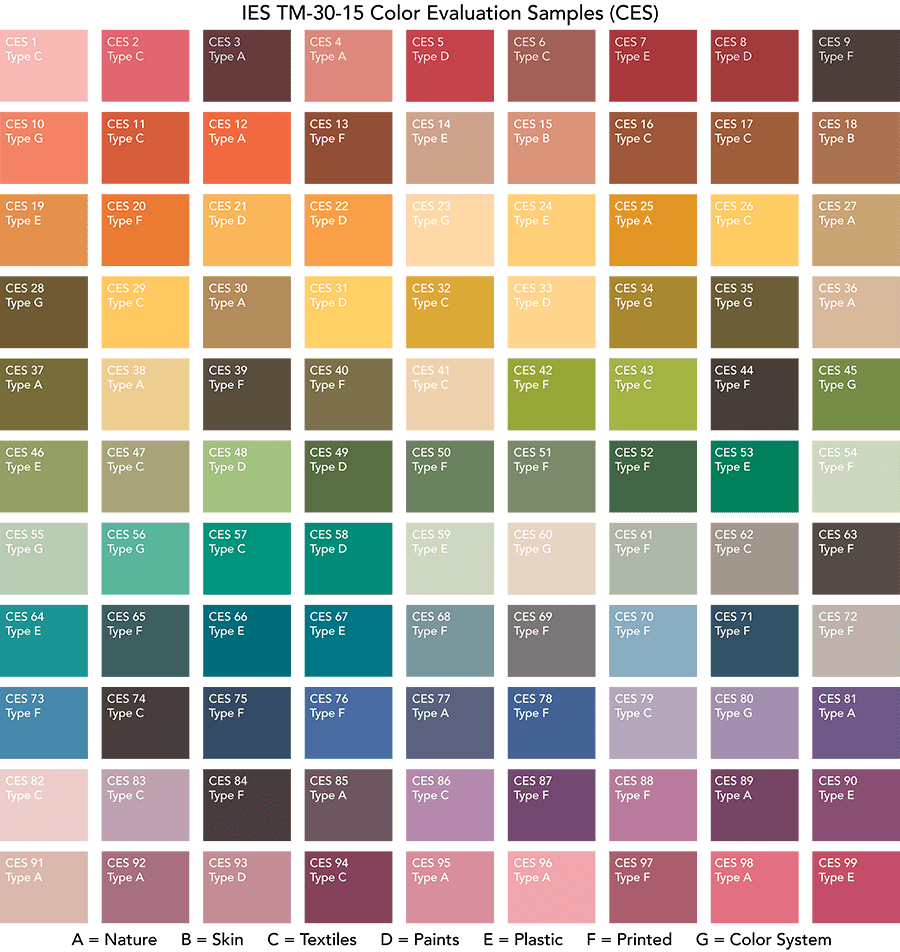
\includegraphics[width=1.0\textwidth]{bilder/tm301} 
% Bilddatei aus dem Unterverzeichnis bilder holen, skalieren auf 0.8*Satzspiegel
\caption {Alle 99 Referenzfarben des TM-30\protect\footnotemark}\label{b_tm301}
\end{figure}
\footnotetext{\url{https://agustos.com/wp-content/uploads/2017/10/TM30-color-samples-image.png}}


Im Gegensatz zum CRI spielen beim TM-30 zwei Werte eine große Rolle: $R_{f}$ und $R_{g}$. Der $R_{f}$-Wert bildet analog zum $R_{a}$-Wert des CRI ein Mittel aus den neunundneunzig Farbunterschieden denen einen Wert von 0 - 100 zugeordnet wird. Auch der $R_{f}$-Wert zeigt nicht an, ob die Leuchte übersättigte Farben hat oder einen Farbshift(\footnote{\cite[10]{royerhouser}}). Dazu wird der $R_{g}$-Wert gemessen. Dieser kann zwischen 60 und 140 variieren und zeigt so, ob die Farben übersättigt ($R_{g} > 100$), untersättigt ($R_{g} < 100$) sind oder mit dem Wert $R_{g} = 100$ genau die Farben der Referenzleuchte (bei selbiger Farbtemperatur) treffen. Mit dem $R_{f}$- und $R_{g}$-Wert wird ein X,Y-Koordinatensystem aufgespannt (Abbildung \ref{b_tm302}). Aus diesem Diagramm sind Farbwiedergabeeigenschaften einer Leuchte sehr gut ablesbar. Durch den zusätzlichen $R_{g}$-Wert gibt es nicht mehr nur Leuchten mit \glqq guter\grqq\ (hoher (hoher $R_{f}$)) oder \glqq schlechter\grqq\ (niedriger $R_{f}$) Farbwiedergabe. Zum Beispiel verliert eine Leuchte mit $R_{f}=82$ und $R_{g}=127$ gegenüber einer mit $R_{f}=90$ und $R_{g}=98$ nicht unweigerlich. Es kommt im direkten Vergleich viel mehr auf den Anwendungsfall an, in der die Leuchte gebraucht wird. Im sterilen Krankenhaus ist eine natürlich Farbwiedergabe wichtig, dort wäre die zweite Leuchte der Favorit, wohingegen für Superläden, in denen das Obst durch Übersättigung der Farben besser zur Geltung kommt, wäre die erste Lampe attraktiver. 
Daher ist der TM-30 viel flexibler zu deuten als der CRI, wo es immer nur um den höchsten $R_{a}$-Wert geht. Eine Möglichkeit könnte es sein, das X,Y-Koordinatensystem in verschiedene Bereiche(z.B. Fenster) einzuteilen, um so anwendungsspezifische Entscheidungen treffen zu können (\footnote{\cite[4]{royer}}).  


\begin{figure}[H]     % h=here, t=top, b=bottom, p=page
\centering
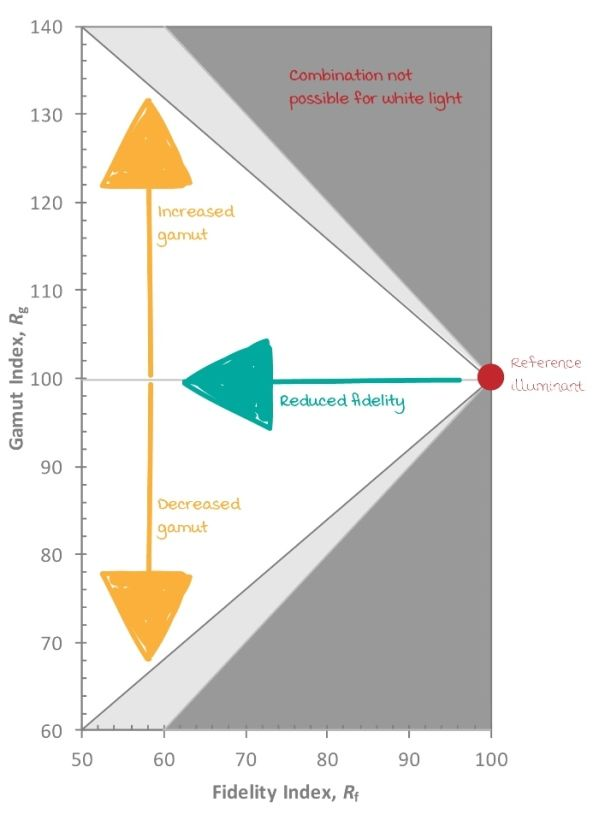
\includegraphics[width=0.5\textwidth]{bilder/tm302} 
% Bilddatei aus dem Unterverzeichnis bilder holen, skalieren auf 0.8*Satzspiegel
\caption {Koordinatensystem aus $R_{f}$ und $R_{g}$: Die hellgraue Zone steht für TM-30-Werte die nicht auf der Plank'schen Kurve liegen und die dunkelgraue Zone steht für alle Werte, die nicht mehr als \glqq weiß\grqq\ angesehen werden. \protect\footnotemark}\label{b_tm302}
\end{figure}
\footnotetext{\url{https://i.pinimg.com/originals/18/98/de/1898de3bdd8436fb5a1945d72a4c6772.jpg}}

In einer anderen Darstellung des $R_{g}$-Wert ist zu sehen, dass der Farbraum in 16 verschiedene \glqq binnings\grqq\ eingeteilt wurde. Jedes dieser \glqq binnings\grqq\ steht übergreifend für die in diesem Bereich liegende Farbtöne. In dieser Darstellung wird mit Pfeilen aufgezeigt, welche Anteile im Farbraum fehlen, welche übersättigt sind und welche den Farbton nicht treffen im Verhältnis zur Referenzfarbwiedergabe (Abbildung \ref{b_tm303}).

\begin{figure}[htp]     % h=here, t=top, b=bottom, p=page
\centering
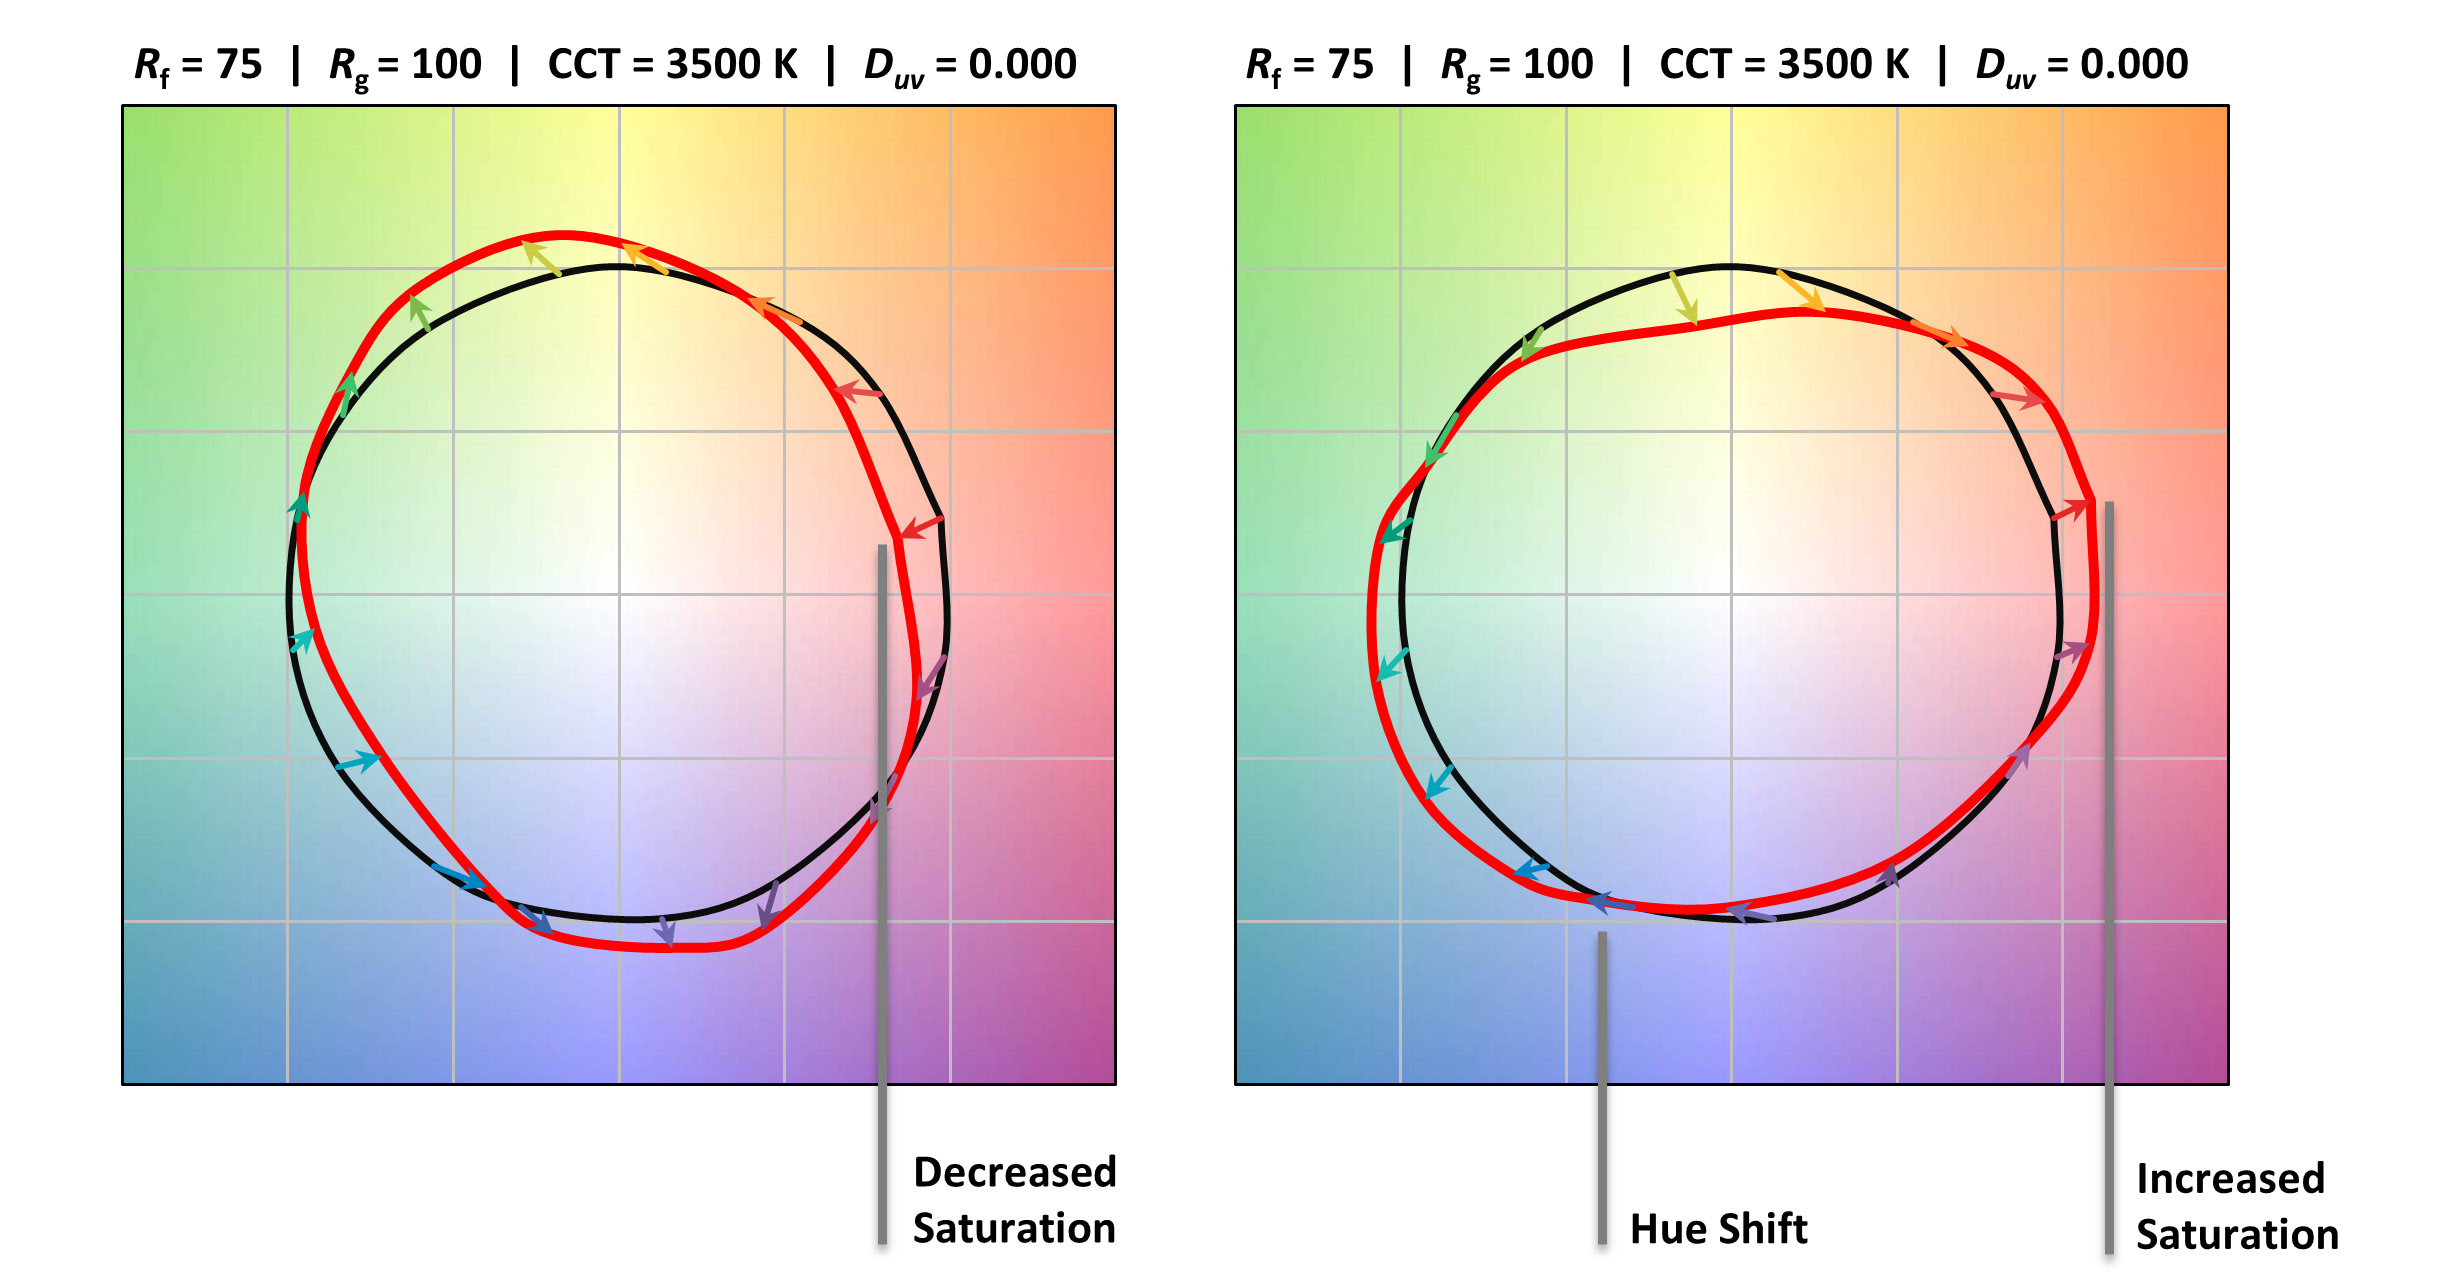
\includegraphics[width=1.0\textwidth]{bilder/tm303} 
% Bilddatei aus dem Unterverzeichnis bilder holen, skalieren auf 0.8*Satzspiegel
\caption {Wie sich die Farben der Testleuchte verhalten ist in der Vektorgraphik des $R_{g}$-Wertes anschaulich dargestellt. Der schwarze Kreis stellt die Referenzleuchte dar, der rote die getestete.  \protect\footnotemark}\label{b_tm303}
\end{figure}
\footnotetext{\cite{usdep}}

Bei der Messung einer Demo warmweiß LED gibt es viel an Messergebnissen zu protokollieren (Abbildung \ref{b_tm304}): Links oben wird gemessene $R_{f}$- und $R_{g}$-Wert angezeigt. Darunter ist die Vektorgraphik des $R_{g}$-Wertes dargestellt und darunter werden die $R_{f}$-Werte der 16 Farbraum-\glqq binnings\grqq\  in einem Säulendiagramm präsentiert. In der Mitte ist der TM-30-Wert in seiner Koordinaten Darstellung aufzufinden und darunter werden die farblichen Abweichungen (in Prozenten) in einem Säulendiagramm dargestellt. Rechts oben wird analog zum TLCI das Spektrum der Leuchte im Verhältnis zum Referenzspektrum gezeigt und die gemessene korrelierte Farbtemperatur angegeben. Darunter gibt es eine Tabelle wo die farblichen Abweichung der einzelnen \glqq binnings\grqq\ als Zahlenwert angegeben werden. Schließlich findet man unter allem bisher genannten eine Säulendiagramm mit allen 99 Farben des TM-30. 
Das Ergebnis einer Messung ist mit diesen Daten nicht mehr schnell ersichtlich, wie beim CRI-Wert, hilft aber eine deutlich aussagekräftigere Entscheidung über eine Leuchte treffen zu können. 

\begin{figure}[H]     % h=here, t=top, b=bottom, p=page
\centering
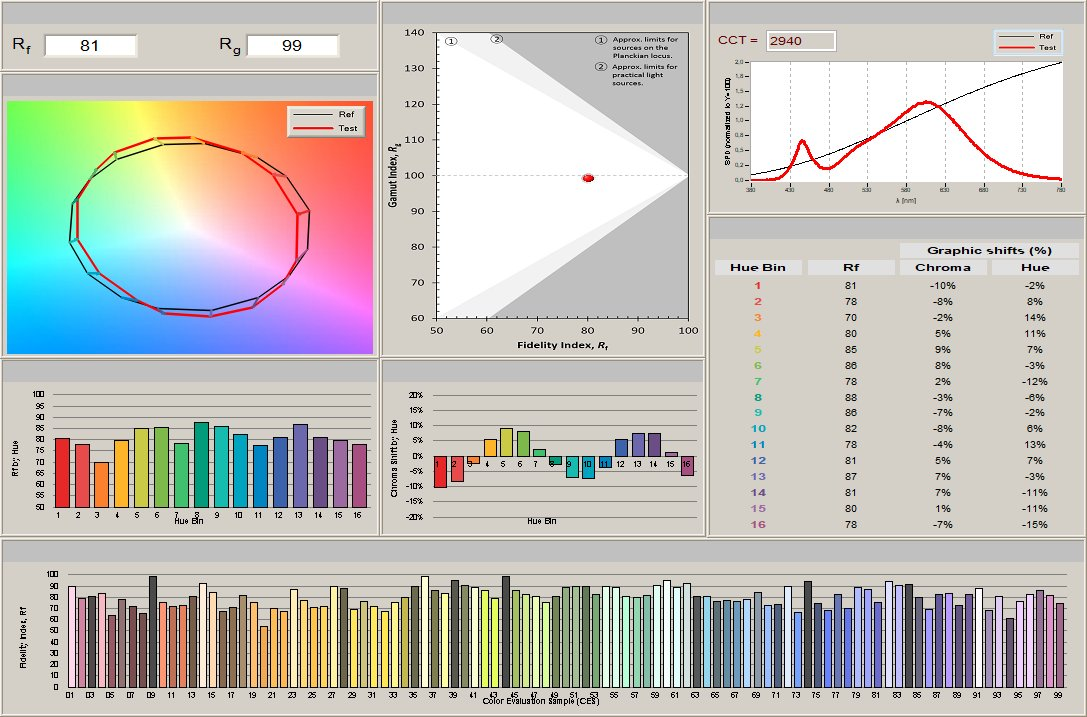
\includegraphics[width=1.0\textwidth]{bilder/tm304} 
% Bilddatei aus dem Unterverzeichnis bilder holen, skalieren auf 0.8*Satzspiegel
\caption {Wie sich die Farben der Testleuchte verhalten ist in der Vektorgraphik des $R_{g}$-Wertes anschaulich dargestellt. Der schwarze Kreis stellt die Referenzleuchte dar, der rote die getestete.  \protect\footnotemark}\label{b_tm304}
\end{figure}

Der TM-30 
%fertig schreiben

\chapter{Messgeräte für Farbmessung}
- Dreibereichsverfahren:
- Licht wird auf drei photoelektrische Empfänger geleitet
- Empfänger sind an durch Filter für die Spektralmeterkurven empfindlich

-Spektralverfahren
 
\section{JETI specbos 1211}

\section{UPRtek M350S}
- CMOS linear image sensor
- diffraction grating um das ankommende Licht im UPRtek aufzuspalten
- licht kommt durch einen leinen spalt ins diffraction grating, wird dort gebrochen und trifft dann auf den CMOS Sensor


\chapter{Grundlagen Videotechnik}

\section{Grundeinstellung einer Kamera}

blende, schärfentiefe, vorverstärkung

\section{Farbbildwandlertechnik einer Kamera}
\label{sec_wandler}
Es gibt verschiedene Arten von Farbbildwandlern, die in einer Kamera verbaut sind. Die gängigsten Methoden sind die 1- und 3-Wandlertechnik. Die Sensoren von \glqq Single Sensor\grqq -Kameras arbeiten mit aufgedampften Bayer Pattern. Herr Dr. Bryce E. Bayer hat sich dabei an der V-$\Lambda$-Kurve des Auges orientiert und daher teilen die Bayer Pattern das Bild in 50\% grüne, 25\% rote und 25\% blaue Pixel auf\footnote{\cite{itwissen}}. Die fehlenden Farbanteile des Bildes werden über die Nachbarpixel interpoliert und diese gesammelten Farbinformationen dann an den Bildwandler weitergegeben (s. Abbildung).
%Bild einfügen

Der Nachteil an dieser Methode ist, dass auf diese Weise die Farbauflösung der Bilder verringert wird. Daher ist eine \glqq Single Sensor\grqq -Kamera nicht geeignet, wenn das entstehende Filmmaterial auf ihre Farbigkeit überprüft werden soll.\\
Bei der 3-Wandler-Technik hingegen wird das in der Kamera ankommende Licht über Filter auf einem Strahlenteiler Prisma in die Farbwertanteile Rot, Grün und Blau aufgespalten und auf den jeweiligen Farbbildwandler durchgelassen\footnote{\cite[378]{schmidt}} (s. Abbildung). 
%Bild einfügen
Da die Filter zur Farbauftrennung nicht ideal sind und vor allendingen blaues Licht auf die nicht dafür vorgesehenen Wandler trifft, gibt es einen weiteren Farbkorrekturfilter vor jedem Wandler\footnote{\cite[379]{schmidt}}. Der Vorteil dieser Variante besteht darin, dass Bild keine Farbauflösung verliert. Die spekrtalen Eigenschaften eines Strahlenteilers zeigen, dass eine Kamera das Licht deutlich anders wahrnimmt, als das Auge (Abbildung).
%Bild einfügen



\section{Weißabgleich}
\label{sec_wb}
Ein Weißabgleich einer Kamera meint den Vorgang eines\emph{\glqq Unbuntabgleich in Bildweiß\grqq} \citep[414]{schmidt}. Unter verschiedenen Beleuchtungssituationen wirkt ein weißes Blatt Papier in der Kamera farbstichig und nicht unbunt. Das liegt daran, das die Kamera erst auf die neue Lichtsituation eingestellt werden muss. Das Auge dagegen kann adaptiert sich meist unbemerkt auf verschiedene Beleuchtungssituationen und so wirkt das Blatt Papier für den Menschen stets weiß. Die Kamera muss also auf Tages- bzw. Kunstlicht geeicht werden, damit in der Kamera weiß auch als solches erkannt wird und keinen Farbstich hat. Ziel ist es bei einem Weißabgleich dass, wenn eine weiße Fläche unter den gewählten Beleuchtungsumständen gefilmt wird, in der Kamera die Signalpegel der RGB-Kanäle zu 100\% ausschlagen. Um die Signalpegel messen zu können, wird das Kamerasignal mit einem Waveformmonitor oder Vektorskop beurteilt (siehe Kaptitel \ref{sec_wmf} und \ref{sec_vector}). Der Vorgang kann in 4 Schritte eingeteilt werden\footnote{\cite[206]{heinen}}:

\begin{enumerate}
\item Die weiße Fläche wird auf mind. 80\% der Bildschirmgröße kadriert, um sicherzustellen, dass wirklich nur die weiße Fläche vom Waveformmonitor erfasst wird.
\item Die Farbtemperatur der Kamera wird über Konversionsfilter im Filterrad nach der Beleuchtungssituation eingestellt. So wird verhindert, dass die Kamera beim Weißabgleich zu stark elektronisch verstärkt wird\footnote{\cite[415]{schmidt}}.
\item Man wählt den Speicherplatz auf der Kamera für den Weißabgleich aus (A oder B). Meist ist es möglich mehrere Weißabgleichdaten zu speichern, um beispielsweise schnell mit der Kamera zwischen Kunst- und Tageslichtsituationen wechseln zu können.
\item Der Weißabgleichsknopf der Kamera wird betätigt und dabei werden die R- und B-Kanäle auf den selben Pegel des G-Kanal verstärkt, sodass alle drei Kanäle den gleichen Signalpegel aufweisen.
\end{enumerate}
  

\section{RGB-Signal}
\label{sec_rgbsignal}
Das unkomprimierte Kamerasignal, dass aus einer Studiokamera kommt, wird RGB-Signal genannt. Es besteht aus den drei Farbwertsignalen R,G und B. Zu diesen Signale ist anzumerken, dass es sich um elektrische Signale mit $\gamma$-Vorverzerrung handelt\footnote{\cite[82]{schmidt}}. Für diese drei Farbwertsignale sind folglich drei Übertragungskanäle nötig. 100\% Signalpegel entspricht einer Übertragungsspannung von $0,7$ V. Damit das transportierte Bild synchron bleibt, wird entweder auf einer separaten Leitung oder auch auf allen drei Leitungen mit einem Signalpegel von $-0,3$ V das Synchronsignal mitgeführt. Das RGB-Signal führt keine Qualitätsverluste mit sich, hat aber einen hohen Bandbreitenbedarf und wird daher nur auf kurzen Strecke im Studio genutzt\footnote{\cite[83]{schmidt}.

\section{Komponenten-Signal}
\label{sec_ycrcb}
Als das Farbfernsehen erfunden wurde, gab es zwei Anforderungen an das Farbfernsehsignal, damit der Übergang vom Schwarz/Weiß-Fernsehen funktioniert: 
\begin{enumerate}
\item Das Farbfernsehsignal muss s/w kompatibel sein. Daher soll Farbfernsehsignal so gestaltet, dass man mit einem Schwarz/Weiß-Fernseher auch fernsehen ohne Farbe kann.
\item Das Farbfernsehsignal soll keine zusätzliche Bandbreite kosten, damit der Fernsehzuschauer zu Hause auch über die s/w Leitung Farbfernsehen empfangen kann
\end{enumerate}

Um diesen beiden Anforderungen gerecht werden zu können, wird das RGB-Signal dementsprechend angepasst. Um die erste Anforderung zu erfüllen, wird aus dem RGB-Signal ein Leuchtdichtesignal errechnet:

\begin{eqnarray}\label{gl_ycrcb1}
	Y = 0,299 \cdot R + 0,587 \cdot G + 0,114 \cdot B\\
	Y = 0,2126 \cdot R + 0,7152 \cdot G + 0,0722 \cdot B
\end{eqnarray}

Die erste Gleichung \ref{gl_ycrcb1} ist für das SD-Signal, die zweite Gleichung für das HD-Signal. Auch hier spricht man wieder von elektrischen Signalen die $\gamma$-vorentzerrt sind. Damit bei einer Bandbreitenreduktion nur die Farbanteile und keine Helligkeiten reduziert werden, wird neben dem Y-Signal auch ein (R-Y)- und (B-Y)- Singal übertragen. Den Farbanteilen wird also das Leuchtdichtesignal abgezogen. Dadurch wie die Helligkeit von den Farbanteilen des Signal getrennt. Es werden absichtlich R und B gewählt, da G-Y nur geringe Pegel ergibt, da Y hauptsächlich durch den Grünanteil bestimmt ist.\\ Die Pegel dieser Farbdifferenzsignale können den maximal Wert von 0,7 V bei Vollausteuerung überschreiten und müssen daher angepasst werden\footnote{\cite[84]{schmidt} (Gleichung \ref{gl_ycrcb2}).

\begin{eqnarray}\label{gl_ycrcb2}
	C_{R}=0,713(R-Y)\\
	C_{B}=0,564(B-Y)
\end{eqnarray}

Diese Gleichungen gelten für SD-Signale. Für HD-Signale sind folgende Gleichungen anzuwenden:

\begin{eqnarray}\label{gl_ycrcb3}
	C_{R}=0,6350(R-Y)\\
	C_{B}=0,5389(B-Y)
\end{eqnarray}


Damit sind die zwei Anforderungen erfüllt. Das $YC_{R}C_{B}$-Signal ist wichtig für die Messung mit dem Vektorskop in den Hauptmessungen (Kapitel). Das Signal an sich muss noch weiter angepasst werden, damit es irgendwann ein sendefähiges Fernsehsignal wird. Diese Entwicklung ist in dieser Arbeit abr nicht mehr von Belang.

%Bild einfügen?


\chapter{Videotechnische Messgeräte}
In der Hauptmessung werden zwei videotechnische Messgeräte genutzt, um den Weißabgleich der Scheinwerfer zu überprüfen und die Farbverschiebung in der Kamera aufzuzeigen.

\section{Waveformmonitor}
\label{sec_wmf}
Ein Waveformmonitor ist ein Oszilloskop für die Videomessung. Oszilloskope basieren auf der Braunschen Röhre mit einem Elektronenstrahl. Dieser wiederum regt einen Bildpunkt auf der Bildschirm des Gerätes an\footnote{\cite[109]{schmidt}}.
Die Messspannung ist für die Ausrichtung des Strahls zuständig und der Elektronenstrahl kann dadurch in horizontaler (x-Achse) wie vertikaler (y-Achse) Ausrichtung beeinflusst werden. Dazu werden zwei Spannungen genutzt (Abbildung) 
%Bild einfügen
Das Messgerät misst eine Zeile des Bildes, die am Gerät ausgewählt werden kann. Bei Messungen wird normalerweise nur die y-Achse genutzt und die horizontaler Richtung wird nach festgelegten Zeit durchlaufen\footnote{\cite[110]{schmidt}}. Auf dem Bildschirm des Messgerätes wird der Pegel von 0-100 angezeigt, so wie der negative Bereich für den Synchonisationbrust bei $-0,3$V. Bei periodischen Signalen wird die Messung speziell getriggert, sodass die Pegelwerte der selben Messzeit und Phasenlänge stets übereinander liegen. Durch bestimmte Filter kann nur das Luminanzsignal, Chrominanzsignal oder beide dargestellt werden\footnote{\cite[111]{schmidt}.\\
Bei einem Weißabgleich werden Waveformmonitore genutzt um zu überprüfen, dass unter einen bestimmen Beleuchtung alle Pegel gleich ausgesteuert sind (Abbildung).

%Bild einfügen


\section{Vektorskop}
\label{sec_vector}
Der Farbton ist mit einem WFM-Monitor nicht gut erkennbar, da der Phasenwinkel der Farbanteilsignale des RGB-Signals im hochfrequenten Bereich schwer auslesbar sind. An dieser Stelle kommt das Vektorskop ins Spiel. Dieses Gerät wird auch mit einen Elektronenstrahl in zwei verschiedene Achsen betrieben. Im Gegensatz zum Waveformmonitor orientiert sich das Vektorskop horizontal an der U- und vertikal an der V-Komponente des FBAS-Signals. Die U- und V-Werte stammen aus dem Farbdifferzsignalen des Komponentensignals mit einer anderen Pegelreduzierung (Gleichung \ref{gl_vector1}.

\begin{eqnarray}\label{gl_vector1}
	U = 0,493(B-Y)\\
	V = 0,877(R-Y)
\end{eqnarray}

Diese Anpassung wird dadurch verursacht, dass die Farbdifferenzsignale im FBAS-Signal in modulierter Form überlagert werden und daher im Pegel reduziert werden müssen\footnote{\cite[84]{schmidt}. Das FBAS-Signal ist eine abgewandelte Form des Komponentensignals und für diese Arbeit unrelevant.\\
Der Bildschirm eines Vektorkops ist mit sechs Toleranzflächen ausgestattet und zeigt über den ganzen Bildschirm alle Farben an. In der Mitte der Anzeige liegt der Unbuntpunkt. Der Elektrodenstrahl fährt über den Bildschirm und zeigt die Farben der Bildzeile an. 


- Auf der Bildschirm flächen werden alle Farben mit Toleranzfeldern angezeigt
- in der mitte liegt unbuntpunkt
- alle 6 Farben sind ständig sichtbar --> abweichung durch toleranzfelder sichtbar
--> winkelabweichung (phasenfehler) --> farbtonfehler 3 prozent toleranz
--> amplitudenabweichung --> Sättigungsfehler 5 prozent toleranz
%bild einfügen
- Vektorskop wird mit Farbbalken und burst kalibriert --> kurze Linie im 135° Winkel
- Elektronenlinie fängt vom 0 Punkt aus an und geht richtung 135° 
- Verstärkung wird dann so gewählt, dass die Länge des Bursts auf 75\% oder 100\% Marke liegt (für jeweilige Farbtafel)

Schmidt S. 112-114
   




\chapter{Vormessungen}

Das Ziel der Hauptmessung ist, das Licht eines 1kW Stufenlinsenscheinwerfers, der mit einem Rosco 027 \glqq Medium Red\grqq\ , Rosco 787 \glqq Marius Red\grqq\ oder Rosco 789 \glqq Blood Red\grqq\ gefiltert wird, mit dem Licht verschiedener LED-Scheinwerfer additiv zu mischen und dem Spektrum des Testscheinwerfers einen \glqq Red Tail\grqq\ anzuhängen. 
Dafür wird in den Vormessungen beobachtet wie stark dieser \glqq Red Tail\grqq\ ausgeprägt sein muss und welche Filter sich für einen \glqq Red Tail\grqq\ eignen.   
Als Beispiel wird der Clay Paky K-Eye K20 representativ für Multichip LED-Scheinwerfer für Personenlicht genommen und der Martin MAC Encore Wash CLD als Gegenstück für reinweiße LED-Engine Scheinwerfer. 
Bei den Rottönen hat man bewusst darauf geachtet, dass sich diese am Rand des Spektrums befinden. Denn Ziel des \glqq Red Tail\grqq\ ist es, dem Spektrum einen tiefroten Anteil anzuhängen, der nicht schon im gelb-orangenen Spektralbereich beginnt und ab dort den gesamtem Spektralbereich erhöht.  

\section{Aufbau und Messungen}
\label{sec_vmaum}

Für die Messung wird der Scheinwerfer direkt neben dem folierten Stufenlinsenscheinwerfer plaziert, um den Messfehler durch unterschiedliche Winkel der Scheinwerfer so gering wie möglich zu halten. Der JETI Specbos 1211, mit dem Standart Diffusor bestückt, wird als primäres Messgerät genutzt. Es wird aus 7m Entfernung direkt gemessen, damit man vergleichbare Helligkeiten erreicht (500lux). 
%Zeichnung einfügen

Den Scheinwerfern wird dann in 10\% Schritten das rotgefilterte Licht des Stufenlinsenschwerfers hinzugemischt. Die Farben des Scheinwerfers werden bei jedem Schritt erneut auf die gleiche Farbtemperatur und gleichem Abstand zum Plank'schen Kurvenzug gedreht, damit die Werte vergleichbar bleiben.


\section{Fazit aus der Vormessung}
\label{sec_vmfazit}
Die Auswirkungen des \glqq Red Tail\grqq\ wird vorallendingen in den TLCI-Werten sichtbar. Zusätzlich sind auch leichte Tendenzen bei den CQS-Werten und den TM-30-Werten bemerkbar.
Wenn man dem K-Eye K20 ein zusätzliches Rosco 027 \glqq Medium Red\grqq\ dazumischt, dann ist der \glqq Red Tail\grqq\ ab 20\% gesättigt. Mit 50\% zusätzlichem Rot sind die Farbwiedergabewerte so niedrig, dass der \glqq Red Tail\grqq\ eine Verschlechterung des Scheinwerfers darstellt. Dies ist eine Folge aus dem Angleichen des Scheinwerferspektrums mit einem größeren \glqq Red Tail\grqq\ .
Das zusätzliche Rot muss jedes mal mit den Farben des Scheinwerfers ausgeglichen werden, um dasselbe 6000k-Weiß zu erhalten. Abhängig von diesem neuen Mischverhältnis mit dem \glqq Red Tail\grqq\ ergibt sich entweder ein Spektrum, dass durch das Rot und die ausgleichenden Farben bereichert wurde, oder das Spektrum wurde durch die stetig größer werdenden Peaks und Einbuchtungen verzogen.
%Bild einfügen


Mit dem Rosco 787 \glqq Marius Red\grqq\ sind analog zum 027 Filter dieselben Tendenzen erkennbar, außer dass die Sättigung des \glqq Red Tail\grqq\ erst bei 30\% erreicht ist.
Der Rosco 789 \glqq Blood Red\grqq\ Filter hingegen zeigt ein anderes Bild. Ab 30\% tritt auch hier die Sättigung des \glqq Red Tail\grqq\ ein. Eine weitere Erhöhung des zuätzliches Rotes ändert aber weder die Farbwiedergabewerte, noch machen sie eine größere Anpassung der Farben des K-Eye K20 nötig. Dieses Verhalten ist daher zu erklären, dass der Transmissionsgrad des Rosco 789 \glqq Blood Red\grqq\ Filters  $Y=1,2\%$ beträgt, also nur 1,2\% des Lichts der Stufenlinsen durchlässt. Dieser selbst gebaute \glqq Red Tail\grqq\ ist mit der Leistungsklasse eines 1kW-Leuchtmittel zu dunkel, um über den Sättigungspunkt hinauszukommen.  

%Bild einfügen

Für den Mac Encore CLD Wash kann man mit dem Rosco 027 \glqq Medium Red\grqq\ eine ähnliche Tendenz wie bei dem K-Eye K20 feststellen. Ab 40\% kann man von einer Sättigung des \glqq Red Tail\grqq\ reden. Der Rosco 787 \glqq Marius Red\grqq\ Filter liefert erst bei 70\% eine Sättigung und zeigt so, dass schon dieser Rotton zu dunkel ist, um die Sättigungswert zu überschreiten. Weil der Rosco 789 \glqq Blood Red\grqq\ Filter noch dunkler als der 787 Filter ist und dieselben Tendenzen wie alle zusätzlichen Rottöne liefert, wird dieser Rotton nicht in den Hauptmessungen verwendet. \\
Die Tendenzen zeigen, dass der \glqq Red Tail\grqq\ vorallendingen den TLCI verbessert und den Scheinwerfern ein besseres kalteweißes Spektrum ermöglicht. In der Hauptmessung wird sich zeigen, wie sich der zusätzliche tiefrote Anteil auf andere Scheinwerfer auswirkt.

%bessere letzte Begründung


\section{Referenzlicht}
\label{sec_reflicht}
Als Referenzlicht ist der Arri Sun 5 mit einem frischen Leuchtmittel bestimmt worden, damit man die LED-Scheinwerfer an dieses Spektrum angeleichen kann. Dieser Scheinwerfer soll durch Abstand und Zoom auch auf eine Beleuchtungsstärke von 500lux gebracht werden. Bei einem größtmöglichen Abstand von 10m ist das nur über den maximalen Zoom des Scheinwerfers möglich. Dies hat zur Folge, dass das Leuchtmittel selbst über den Reflektor des Scheinwerfers gespiegelt und \glqq rückprojeziert\grqq\ wird, dass dadurch ein dunkler Bereich in Mitten des Lichtkegels entsteht. Da man das Referenzspektrum nicht verfälschen möchte, wird bei dem Referenzlicht auf jegliche Art von Filtern verzichtet. Unter dieses Umständen kann der Arri Sun 5 nicht als Referenzlampe genutzt werden.

Daher wird in der Hauptmessung ein Arri True Blue D5 genutzt, der innerhalb von 10m, mit dem Zoom auf 500 lux angepasst, ein gutes Referenzlicht liefert, allerdings ca. 600K wärmer als der Arri Sun 5 ist. So kommt es, dass die Vormessungen auf 6000K, die Hauptmessung jedoch auf 5400K eingemessen sind. Da nur die Tendenzen der Vormessung eine Rolle spielen und die Vormessung keine direkte Einwirkung auf die Hauptmessung hat, ist dieser Unterschied zu vernachlässigen.

%Referenzlicht bild einfügen

\chapter{Hauptmessung}
Für die Hauptmessungen werden vier Scheinwerfer mit Multichip-LED Engine und zwei Scheinwerfer mit reinweißer LED-Engine ausgewählt. Bei den Multichip-Scheinwerfer ist der zuvorgenannte Clay Paky K-Eye K20, mit 6 verschieden farbigen LEDs, dabei, als Alternative, der Robe Robin Dl7F Wash, mit 7 verschieden farbigen LEDs, und der weltweit verbreitete ETC Source Four LED Series 2 Lustr, ebenfalls mit 7 verschieden farbigen LEDs. Dazu kommt eine weiterer \glqq Standartscheinwerfer\grqq\ aus dem TV-Bereich: der GLP Impression X4 in der \glqq L\grqq\ - Variante. Dieser verfügt über eine rote, grüne und blaue, wie eine weiße LED in seinen LED-Arrays. Weiterhin gab es noch den Martin MAC Encore CLD Wash speziell für die Personenbeleuchtung ausgelegt mit einer reinweißen LED-Engine und den Ayrton Ghibli, ebenfalls mit einer reinweißen LED-Engine, als Beispiel für einen LED-Effektscheinwerfer. 
Mit diesen Scheinwerfern soll die Auswirkung eines \glqq Red Tail\grqq\ überprüft werden.



\section{Messaufbau und Messungen}
\label{sec_hmaufbau}
Der Messaufbau gleicht dem der in der Vormessung (Kapitel \ref{sec_vmaum}). Mit 7m Abstand werden die Scheinwerfer zum Messgerät aufgebaut und über Zoom- und Abstandsvariation auf ca. 500 lux Beleuchtungstärke eingestellt, nachdem sie auf das Arri D5-Referenzweiß abgeglichen worden sind. Es wird wiederum mit dem JETI specbos 1211 mit dem Standartdiffusor gemessen und mit dem UPRtek M350S gegenkontrolliert. Alle Scheinwerfer werden so nahe wie möglich an den 1kW Stufenlinsenscheinwerfer mit den roten Filterfolien herangestellt, um den Fehler der verschiedenen Winkel so gering wie möglich zu halten. Der zu messende Scheinwerfer ist dabei im rechten Winkel zum Messgerät angeordnet, der Stufenlinsenscheinwerfer leicht angewinkelt. 

%Bild einfügen

Jeder Scheinwerfer wird also auf eine Farbtemperatur von 5395K des Referenzlichts eingestellt, mit einem möglichsten geringen Abstand zur Plank'schen Kurve ($ \Delta u'v'=\pm0,0001$) und einem sehr ähnlichem Farbort, um die Messungen vergleichbar zu machen. Wenn dem Scheinwerfer ein \glqq Red Tail\grqq\ hinzugemischt wird, wird der Scheinwerfer erneut auf die Referenz angeglichen. 

%zuwenig?

\chapter{Messergebnisse}

Die Tendenzen zeigen, dass der Ghibli, MAC Encore, Lustr und K-Eye K20 durch den Red Tail verbessert wurden. Wie in den Vormessungen zu sehen, zeigt sich dies in allen Farbwiedergabewerten, vorallendingen aber im TLCI. Der MAC Encore kann mit einem Rosco 027 \glqq Medium Red\grqq\ im TLCI sogar um 16 Punkte verbessert werden. Diese Scheinwerfer zeigen, dass der zusätzliche \glqq Red Tail\grqq\ eine Verbesserung des Spektrums darstellt, unabhänging davon, welches zusätzliche rot genutzt wird. 
% Bild einfügen

Die Erklärung liegt hier wie in der Vormessung an den beiden Vorteilen des \glqq Red Tail\grqq\ : Es wird auf der einen Seite der tiefrote Bereich der Scheinwerfer aufgefüllt und zum anderen werden zum Ausgleich des zusätzlichen tiefroten Anteils wieder wertvolle Anteile in der Mitte des Spektrums dazugemischt. Spannend ist, das beim Clay Paky K-Eye K20 nur der TLCI verbessert werden konnte. Dies hängt damit zusammen, dass dem K-Eye K20 mit \glqq Red Tail\grqq\ deutlich weniger Amber zur Verfügung steht und der 645nm Rot-Peak in die Höhe schießt. Das Spektrum wird also unausgeglichener und dafür von den Farbwiedergabewerten bestraft.\\
%Verweis einfügen
Der Impression X4L konnte nicht durch ein zusätzliches rot verbessert werden. Dies liegt daran, dass das Spektrum, des X4Ls vorallendingen aus schmalbandigen Peaks besteht, die das Spektrum nicht ausfüllen. Zusätzlich kann man mit der blauen LED, das Spektrum nicht weiter ausfüllen, da der Peak der weißen LED exakt mit dem der blauen LED übereinstimmt. Auch ein Angleichen des Spektrums mit einem \glqq Red Tail\grqq\ verbessert dieses extreme Spektrum nicht, sondern vergrößert das spektrale Tief im 595nm Wellenlängebereich sogar. Ein aufgefülltes Spektrum kann also mit einem \glqq Red Tail\grqq\ bereichert werden, während man bei einem schmalbandigen Spektrum für eine Auffüllung der Randbereiche nicht belohnt wird.\\
%Bild einfügen
Bei dem Robe Robin DL7F haben wir im High-CRI Modus auch keine Verbesserung mit einem \glqq Red Tail\grqq\ erzielen können. Das Spektrum des Robin DL7F ist durch viele Peaks und Täler gekennzeichnet, außer im Bereich von 510nm-550nm Wellenlänge, wo das Spektrum sehr breitbandig ist. Durch Angleichungen an den \glqq Red Tail\grqq\ wird das Lime vermindert, das Tal im gelben Spektralbereich noch tiefer und der rot Peak wird erhört. Das Spektrum wird also noch mehr in seine Extreme verzerrt und dass wird von den Farbwiedergabewerten bestraft.
%Bild einfügen

\section{Analyse der Farbwiedergabewerte}
\label{sec_analfww}
Die Farbwiedergabewerte haben unterschiedlich stark auf den \glqq Red Tail\grqq\ reagiert. Der TLCI zeigt dabei stets den größten Ausschlag mit bis zu 16 Punkten, CQS und TM-30 erhöhen sich höchsten um 5 Punkte. Dies verwundert bei einem TM-30, der mit seinen 99 Farben folglich keine tiefrote Referenz besitzt. Jedoch ist die Verbesserung des Rotanteils stehts im roten \glqq binning\grqq\ zu erkennen(s. Kap. \ref{sec_tm30}). Ebenso ist im CQS am 1. Referenzwert der dazugekommene  
%fertig schreiben und vernünftig angucken !!


\section{Fazit aus den Hauptmessungen}
\label{sec_fazithm}
Aus den Hauptmessungen lässt sich schließen, dass der \glqq Red Tail\grqq\ tendenziell die Scheinwerfer verbessert. Am deutlichsten ist dies stets im TLCI zu erkennen, es macht sich aber ebenso im CQS, wie im TM-30 bemerkbar. Die Verbesserung ist einmal durch den zusätzlichen tiefroten Anteil im Spektrum zu erklären und dadurch, dass das Spektrum mit diesem neu angepasst wird. Bei Scheinwerfern mit schmalbandigen Spektren führt der Red Tail dazu, dass die Spektren noch extremer werden (größere Peaks, größere Täler) und so können die Farbwiedergabewerte nicht verbessert werden. Ein zu großer \glqq Red Tail\grqq\ ist nicht zu empfehlen, da es die Farbwiedergabewerte des Scheinwerfers wieder verschlechtern würde (siehe Kap. \ref{sec_vmfazit}). Daher sollte für jeden Scheinwerfer ein \glqq Red Tail\grqq\ individuell ausbalanciert werden.




\chapter{Umfrage}

\section{Anpassung der Scheinwerfer}
\label{sec_anpassunglampen}
Der nächste Schritt ist, auch über eine Kamera zu prüfen, welche Auswirkung der \glqq Red Tail\grqq\ auf das Spektrum der Scheinwerfer hat. Dazu sollen Probanden verschiedener Hauttöne mit und ohne \glqq Red Tail\grqq\ beleuchtet werden und dabei mit einer Kamera abgefilmt werden. Die so entstandenen Bilder werden dann in einer Umfrage miteinander verglichen.\\
Da eine Kamera das Spektrum eines Scheinwerfer deutlich anders bewertet als der JETI specbos 1211 (s. Kap ), gibt es drei Möglichkeiten fortzufahren:

\begin{enumerate}\setlength{\itemsep}{0ex}
\item Weißabgleich durch Scheinwerfer: Man gleicht die Kamera auf das Referenzweiß des Arris ab und dreht alle Farben der Scheinwerfer so hin, dass diese in der Kamera weiß erscheinen.
\item Weißabgleich durch Kamera: Man gleicht für jedes Bild die Kamera neu auf den Scheinwerfer an.
\item kein Weißabgleich: Man gleicht die Kamera auf das Referenzweiß des Arris ab und verwendet danach die Farbwerte der Scheinwerfer, so wie sie mit dem JETI specbos 1211 hingedreht worden sind.
\end{enumerate}

Variante 1 macht den Bezug zu den Messwerten des JETI specbos 1211 kaputt, da die auf die Kamera angepassten Scheinwerfer dann nicht mehr die selbe Farbtemperatur, den selben Abstand zu Plank'schen Kurve oder einen ähnlichen Farbort haben. Variante 2 erhält diese Werte, aber es kann nicht mehr wissenschaftlich beschrieben werden, welche Veränderung die Kamera durch den Weißabgleich am Spektrum vornimmt. So kann nicht mehr unterschieden werden, ob die Kamera nun aus dem Licht das natürlichere weiß gemacht hat, oder dies tatsächlich eine Auswirkung des \glqq Red Tail\grqq\ ist.
Variante 3 ist abzulehnen, weil die vermeintlich gleichen Lichtverhältnisse durch den JETI specbos 1211 gemessen durch die Kamera nicht als ähnliches weiß gesehen werden. Die Spektren der Scheinwerfer sind sehr unterschiedlich und werden daher auch von der Kamera so wahrgenommen.

Der Vollständigkeit halber werden alle 3 Varianten aufgezeichnet. Für die Umfrage hat man sich für die erste Variante entschieden, da ein typischer Weißabgleich im TV-Bereich genauso abläuft. Zuerst wird ein Scheinwerfer als Referenzlicht bestimmt und alle anderen Scheinwerfer werden mit der Kamera auf dieses Weiß korrigiert. 

Zu Demonstrationszwecken wird mit dem Mac Encore Wash CLD und dem K-Eye K20 mit einer Farbtafel aufgezeichnet. Über ein Vektorskop ist deutlich sichtbar, was die verschiedenen Varianten für Auswirkungen auf die Farben in der Kamera haben. Dies ist jedoch für diese Arbeit irrelevant und wird an dieser Stelle nicht weiter ausgeführt. %Anhang aufführen

\section{Auswahl der Kamera und der Probanden}
\label{sec_wahlderKamera}

Die Kamerawahl trifft auf eine Sony HDC-4300 UHD mit Weitwinkelobjektiv. Diese Kamera nutzt drei Bildwandler und keinen Bayer-Sensor. Bei einem Bayer-Sensor wird das Bild in 50\% Grünanteil 25\% Rotanteil und 25\% Blauanteil aufgeteilt. Nur diese Farbanteile werden vom Sensor gespeichert, die restlichen 50\% Grünanteile und 75\% Rot- und Blauanteile des Bilders werden aus den Nachbarpixeln interpoliert. Die Folge daraus ist eine niedrigere Farbauflösung als mit 3 Bildwandlern\footnote{\cite[380-381]{schmidt}}. Da die Bilder auf ihre Farbigkeit verglichen werden sollen, wird sich bewusst für eine Kamera mit drei Bildwandlern entschieden(siehe Kaptitel \ref{sec_wandler}).\\

Die Probanden werden nach möglichst unterschiedlichen Hauttönen ausgewählt. Leider sind am Aufnahmetag nicht alle Probanden erschienen und daher ist die Bandbreite der Hauttöne nicht so groß wie erhofft, aber dennoch aussagekräftig genug, um die Auswirkung des Red Tail beurteilen zu können. Denn nach Khan (Kap.)ist jeder Hauttyp stark im roten Spektralbereich vertreten. Die Probanden haben einen nordischen, einen südländischen, einen normalen und einen braun-gebrannten Hauttyp. /%Bild einfügen

 
\section{Erstellung der Bilder}
\label{sec_erstellungbilder}
Bei der Erstellung der Bilder werden die Probanden auf selber Augenhöhe nebeneinander gestellt. In der Mitte steht eine Graustufenkarte für den Weißabgleich. Nachdem die Scheinwerfer und Kamera angepasst sind, wie in Kapitel \ref{sec_anpassunglampen} beschrieben, werden die Probanden für 10 Sekunden gefilmt. Dabei wird am Anfang der Aufzeichnung ein Tablet mit den aktuellen Einstellungen der Scheinwerfer und Kamera gezeigt, damit später die Daten eindeutig zugeordnet werden können.\\
Nach den Aufzeichnungen mit den Probanden wird, nochmal die Graustufenkarte für jede Einstellung einzeln aufgezeichnet, damit man auf dem Waveformmonitor das Weiß der Scheinwerfer messen kann. Durch diesen Ablauf sind Messungenauigkeiten bei der Aufzeichnung des Waveformmonitors möglich. 

\section{Umfrage nach Rec. ITU-R  BT.500-11}
\label{sec_umfrageitu}
In der \glqq Recommendation ITU-R BT.500-11: Methodology for the subjective assessment of the 
quality of television pictures\grqq\ werden verschiedene Vorgehensweisen beschrieben, wie man die Qualität von Fernsehbildern durch Umfragen einschätzen kann. Je nach dem welches Bildmaterial man zur Verfügung hat und welche Aussage man untersuchen möchte, empfiehlt die ITU-R eine andere Methode. Da der Arri D5 zwar die Referenzleuchte für den Weißabgleich ist, aber die Scheinwerfer nicht mit diesem verglichen werden soll, wird entschieden, nach der \glqq Ratio-scaling method\grqq\ vorzugehen\footnote{\cite[10]{itu}}, eine Methode ohne Refernz. Diese findet man wiederum in dem \glqq Report ITU-R BT.1082\grqq\ von 1990 und funktioniert wie folgt:
Den Probanden werden in zufälliger Reihenfolge Bilder gezeigt. Jedes  Bild soll nach dessen Qualität beurteilt werden. Dabei wird den Probanden aber keine Skala zur Bewertung vorgegeben. Der Proband entscheidet selbst, wie er seine Skala wählt. Dazu vergibt er dem ersten Bild einen ersten Eindruck in einer Zahl ausgedrückt. Je nachdem ob ihm das darauffolgende Bild besser oder schlechter befindet, wählt er die Zahl für das zweite Bild größer, kleiner (oder gleich) der ersten Zahl. Bei der Skalierung sind dem Probanden keine Grenzen gesetzt. Wenn er ein Bild dreimal so gut wie das erste befindet, kann er dem Bild den dreifachen Wert des ersten Bildes geben. Falls Bild Nummer drei zwischen der Qualität von Bild eins und zwei liegt, darf der Proband auch mit Brüchen oder Nachkommastellen einen Wert zwischen der Zahl ein und zwei finden. Der Vorteil dieser Methode ist, das die Probanden nicht an eine vorgegebene Skala gebunden sind und mit dieser nur bestimmen, wie gut Bilder sind, sondern mit dieser freien Skala auch festlegen können, um wie viel ein Bild besser oder schlechter ist\footnote{\cite[385]{itu90}}. Um die Bewertung der Bilder verschiedener Probanden nun miteinander vergleichen zu können, müssen die vergebenen Zahlen x auf die beste Bewertung $R_{1}$ des Probanden normiert werden\footnote{\cite[387]{itu90}} (Gleichung \ref{gl_umfrage}).

\begin{equation}\label{gl_umfrage}
		X_{norm} = x \cdot \frac{100}{R_{1}}
\end{equation}
Da die Probanden nur Tendenzen mit ihren Zahlen aufzeigen, sind die einzelnen Werte $X_{norm}$ der Bilder in der Auswertung der Umfrage nicht eins zu eins vergleichbar, sondern nur mit ihr Tendenz zu den anderen Bildern zu betrachten.

\section{Aufbau und Durchführung der Umfrage} 
Die Umfrage wird in einem abgedunkelt Raum durchgeführt. Der Klasse 1 Monitor wird mit dem Jeti Specbos 1211 auf $100\frac{cd}{m^{2}}$ Leuchtdichte eingemessen und auf den Farbort der Normlichtart D65 angeglichen. Das Umgebungslicht wird mit einem Arri L7-C simuliert und  auf eine ähnliche Farbtemperatur eingestellt, damit sich die Probanden auf den kalten Bildschirm adaptieren.\\
Dem Proband wird das Verfahren aus Kapitel \ref{sec_umfrageitu}  erklärt und dann werden ihm alle Bilder zwei mal in einer zufälligen Reihenfolge gezeigt, wie von dem \glqq Report ITU-R BT.1082\grqq\ empfohlen \footnote{\cite[368]{itu90}}. Der Teilnehmer soll das einzelne Bild auf seine Natürlichkeit untersuchen und mit einer Zahl bewerten. Für jedes der 38 Bilder hat der Proband 10 Sekunden Zeit. Er kann den Ablauf jederzeit stoppen, um sich seine Zahl zu notieren, darf aber die Bilder nicht vor oder zurückschalten, da sonst die Tendenzen der Bilder kaputt gehen. Die ITU hält 15 Teilnehmer an der Umfrage für ausreichend\footnote{\cite[368]{itu90}}. Dies liegt daran, dass es nicht darum geht, ein Ergebnis bezüglich einer bestimmten Bevölkerungsgruppe zu generieren. Ziel der Umfrage ist es lediglich festzustellen, welche Auswirkung der \glqq Red Tail\grqq\ auf die optische Natürlichkeit des Bildes hat, ohne speziellen Bezug zu den Probanden. So reichen deutlich weniger Teilnehmer, als bei teilnehmerspezifischen Umfragen. Um die Statistik zu festigen haben 20 Probanden an der Umfrage teilgenommen. Eine Durchführung der Umfrage dauert ca. 15 Minuten.

% Bild einfügen
%mit Wilkens über D65 einstellung reden

\chapter{Umfrageergebnisse}
Die Tendenzen der Umfrage lassen erkennen, dass die Probanden die gezeigten Hauttöne, mit einem \glqq Red Tail\grqq\ beleuchtet, als natürlicher befinden. Dieses Verhalten zeigen die Kurven des Source Four LED Series 2 Lustr, des MAC Encore Wash CLD und des K-Eye K20. %Grafik einfügen
Dies liegt zum einen daran, dass der zusätzliche tiefrote Anteil das Spektrum auffüllt, wo es für die Hauttöne wichtig ist. %Referenz zu Khan
Zum anderen hilft die Anpassung an den \glqq Red Tail\grqq , dass Spektrum einwenig aufzufüllen und das Peak-Loch-Verhältnis des Scheinwerfers anzupassen. Daher werden die Bilder mit einem \glqq Red Tail\grqq\ nicht rotstichiger, sondern sie wirken durch die Anpassung eher so, wie man es in der Natur erwarten würde.
%Grafik einfügen

Das extreme Spektrum des Impression X4L sticht aus der Bilderreihe hervor und wirkt auf den Bildern rotstichig. Bei der Umfrage ist dieses Spektrum (mit oder ohne \glqq Red Tail\grqq) mit Abstand am besten bewertet worden. Das lässt sich darauf zurückführen, dass die Probanden ans Glühlicht gewöhnt sind. Blau- oder grünstichige Bilder von Menschen wirken krank und unnatürlich. Dagegen wirken rotstichige Bilder nicht falsch, da Menschen unter Glühlicht auch rötlicher aussehen. Außerdem wird die menschliche Haut röter, wenn man in der Sonne liegt. Man ist es also durchaus gewohnt, dass Hauttöne rötlich erscheinen und dadurch werden die Bilder des Impression X4L auch als natürlich gesehen. 
%Grafik einfügen

Beim Robin DL7F ist beim dritten Bild mit dem Rosco 787 \glqq Marius Red\grqq\ ein kaputtes Bild in der Umfrage gelandet. Es ist deutlich sichtbar, dass die Kamera die Probanden zu hell darstellt und dadurch die Hauttöne sehr unnatürlich aussehen. Daher ist dieser Wert für die Umfrage ungültig. Dennoch haben die Probanden dieses Bild auch durchgehend schlecht bewertet und somit zeigt sich, dass das Verfahren des\glqq Report ITU-R BT.1082\grqq\ funktioniert. 
Wenn man dem Ghibli ein Rosco 027 \glqq Medium Red\grqq\ dazumischt, und die Werte wieder auf den Ghilbi anpasst zeigen die Hauptmessung eine Verbesserung der Werte. Dagegen wirken die Probanden bei der Umfrage matt und krank und es ist keine Verbesserung sichtbar. Dies liegt am Spektrum des Ghibli, der mit seiner reinweißen LED-Engine Probleme hat, das Spektrum auszufüllen. Dem Ghibli wäre deutlich besser geholfen, wenn man das Loch im Spektrum von 470 nm bis 510 nm Wellenlänge und den Rotbereich des Spektrums aufbessern würde. Nur einen tiefroten Anteil zu ergänzen reicht nicht aus, und das macht sich auch optisch bemerkbar.\\
Vielen Probanden ist es schwer gefallen die Bilder einzuschätzen, da sich der rechte nordische Hauttyp deutlich von den anderen Hauttypen unterscheidet. Daher ist es zu einem Konflikt in der Entscheidung gekommen, wie das Bild zu beurteilen sei, wenn der helle Hautton auf dem Bild natürlich wirkte, nicht aber die anderen Hauttypen. Anderen Probanden wiederum hat dieser Unterschied geholfen, die Bilder besser einschätzen zu können. Da die vorgeschlagene Länge einer Umfrage in dem \glqq Report ITU-R BT.1082\grqq\ eine halbe Stunde nicht überschreiten sollte hat man sich für den Vergleich aller Hauttypen gleichzeitig entschieden. Ansonsten vervierfacht sich die Anzahl der 38 Bilder und damit erhöht sich die Länge der Umfrage auf eine Stunde. 




\chapter{Fazit}
Sowohl im messtechnischen als auch im optischen Vergleich konnte mit dem \glqq Red Tail\grqq\ das Licht tendenziell verbessert werden. Dieses Verhalten zeigt sich vorallendingen beim TLCI um bis zu 16 Punkten. Ein zusätzlicher tiefroter Anteil verbessert den Scheinwerfer, wie in Kapitel \ref{sec_fazithm} dargestellt, auf der einen Seite durch den zusätzlichen Rotanteil und auf der anderen Seite durch die Anpassung an den \glqq Red Tail\grqq\ . Spektren, die sehr durch Peaks geprägt und / oder schmalbandig sind, können durch einen zusätzlichen tiefroten Spektralanteil nicht verbessert werden, da die Anpassung das Spektrum der Scheinwerfer noch extremer werden lässt (s. Daten von GLP und DL7F). Auch optisch stellt der \glqq Red Tail\grqq\ dort keine Verbesserung dar. Der Ghibli kann zwar messtechnisch verbessert werden, dies konnte aber nicht in der Umfrage festgestellt werden, weil sein Spektrum sich nicht besonders gut dafür eignet, Personen zu beleuchten. Ein TLCI von 50 zeigt dem Coloristen in der Nachbearbeitung, dass die \glqq Aufbereitung sehr zeitaufwendig\grqq\ sein wird (Kapitel \ref{sec_tlci}). Daher konnte der Ghibli optisch nicht überzeugen.\\
Die Bilder sind alle mit einer Sony HDC-4300 UHD mit Weitwinkelobjektiv aufgezeichnet worden. Die Wirkung der Bilder sollte daher mit anderen Objektiven und Kameras überprüft werden. Auch bei anderen Hauttypen und Scheinwerfer gilt es den \glqq Red Tail\grqq\ zu untersuchen. Der zusätzliche tiefrote Spektralanteil bei einem LED-Scheinwerfer muss also immer im Zusammenhang mit dem Spektrum des Scheinwerfers, der filmenden Kamera und der zu beleuchtenden Hauttöne gesehen werden. Die Tendenzen dieser Arbeit zeigen unter der Berücksichtigung der genannten Parameter, dass der \glqq Red Tail\grqq\ den Scheinwerfer messtechnisch verbessert und optisch Hauttöne natürlicher aussehen lässt.

  


\chapter{Ausblick}

\section{Unterkapitel mit Mathematik, Bildern und Querverweisen}





%--------------------- VERZEICHNISSE ----------------

\listoffigures % Abbildungsverzeichnis erzeugen
\listoftables % Tabellenverzeichnis erzeugen

%--------------------- LITERATURLISTE ---------------
% Die Einträge sollen alphabetisch sortiert sein.

\begin{thebibliography}{}

% Formatierung für Internetquelle
% Grundregel: Name, Vorname (falls vorhanden), VÖ-Jahr (falls vorhanden), Titel in Anführungszeichen, URL, Datum des letzten Aufrufs
% zur Formatierung der URL unbedingt den url-Befehl benutzen!!!

\bibitem[ITWissen.info(2017)]{itwissen}
ITWissen.info:
\emph{\glqq BAyer-Filter\grqq}
\url{https://www.itwissen.info/Bayer-Filter-bayer-filter.html}, 09.05.2017, letzter Zugriff 10.08.2018

\bibitem[Bladowski \& Maus(2010)]{unimann}
Bladowski, Beate \& Maus, Daniel:
\emph{\glqq Farbwahrnehmung\grqq}
\url{http://irtel.uni-mannheim.de/lehre/seminararbeiten/w96/Farbe/seminar.htm#Wieviele}, 15.07.2010, letzter Zugriff 28.06.2018

\bibitem[Royer \& Houser(2015)]{royerhouser}
Royer, Micheal \& Houser Kevin:
\emph{\glqq Understanding and Applying TM-30-15\grqq}
\url{https://www.energy.gov/sites/prod/files/2015/09/f26/tm30-intro-webinar_9-15-15.pdf}, 15.09.2015, letzter Zugriff 26.06.2018

\bibitem[U.S. Department of Energy(2015)]{usdep}
U.S. Department of Energy:
\emph{\glqq Evaluating Color Rendition Using IES TM-30-15\grqq}
\url{https://www.energy.gov/sites/prod/files/2016/04/f30/tm-30_fact-sheet.pdf}, Oktober 2015, letzter Zugriff 25.06.2018

\bibitem[Commission Internationale de l'Eclairage(2007)]{CIE}
Commission Internationale de l'Eclairage:
\emph{\glqq Technical Report 177:2007 : Color Rendering of White LED Light Sources\grqq}
\url{https://de.scribd.com/document/125319182/CIE-177-2007}, 2007, letzter Zugriff 20.06.2018

\bibitem[Davis \& Ohno(2006)]{davis_ohno}
Davis, Wendy L. \& Ohno, Yoshihiro:
\emph{\glqq Development of a Color Quality Scale\grqq}
\url{http://citeseerx.ist.psu.edu/viewdoc/download?doi=10.1.1.568.8399&rep=rep1&type=pdf}, 08.02.2006, letzter Zugriff 20.06.2018

\bibitem[DocCheck Flexikon(2014)]{doccheck sko}
DocCheck Flexikon:
\emph{\glqq Skotopisches Sehen\grqq}
\url{http://flexikon.doccheck.com/de/Skotopisches_Sehen}, 24.01.2014, letzter Zugriff 18.06.2018

\bibitem[DocCheck Flexikon(2014)]{doccheck pho}
DocCheck Flexikon:
\emph{\glqq Photopisches Sehen\grqq}
\url{http://flexikon.doccheck.com/de/Photopisches_Sehen}, 10.05.2016, letzter Zugriff 18.06.2018

\bibitem[Production Partner(2018)]{production partner}
Production Partner:
\emph{\glqq Farbwiedergabe: TM-30-15, CRI und Co.\grqq}
\url{https://www.production-partner.de/basics/farbwiedergabe-tm-30-15-cri-und-co/}, 22.02.2018, letzter Zugriff 20.06.2018

\bibitem[Gigahertz-Optik(2012)]{Gigahertz}
Gigahertz-Optik:
\emph{\glqq Grundladen der Lichtmesstechnik\grqq}
\url{https://www.gigahertz-optik.de/de-de/grundlagen-lichtmesstechnik/}, letzter Zugriff 20.06.2018


% Formatierung für Aufsatz / Paper: Titel in Anführungszeichen, Zeitschriftentitel kursiv
\bibitem[Ohno(2005)]{ohno} 
Ohno, Yoshi:
\glqq Spectral design considerations for white LED color rendering\grqq, 
\emph{Optical Engineering} vol. 44 (11), November 2005


\bibitem[Jiajie \& Yung \& Pecht(2014)]{jiyupe} 
Fan, Jiajie \& Yung, Winco \& Pecht, Michael:
\glqq Prognostics of Chromaticity State for Phosphor-Converted White Light Emitting Diodes Using an Unscented Kalman Filter Approach\grqq, 
\emph{Device and Materials Reliability} vol. 14, 01.03.2014

\bibitem[Royer(2016)]{royer} 
Royer, Michael P.:
\glqq IES TM-30-15 Is Approved—Now What?\grqq, 
\emph{LEUKOS} vol. 12 (1-2, 3-5), 2016


\bibitem[Dooley \& Streicher(1982)]{dooley_streicher} 
Dooley, Wesley L.  \& Streicher, Ronald D.:
\glqq M--S Stereo: A Powerful Technique for Working in Stereo\grqq, 
\emph{Journ. Audio Engineering Society} vol. 30 (10), 1982

% Formatierung für Fachbuch, Diplomarbeit o.Ä.: Titel kursiv
\bibitem[Heinen(2012)]{heinen}
Heinen, Gerd: 
\emph{AV-Medientechnik}, 1. Aufl., Europa-Lehrmittel 2012

\bibitem[Roberts(2015)]{roberts}
Roberts, Alan: 
\emph{TELEVISION LIGHTING CONSISTENCY INDEX (TLCI-2012)}, Version 2.015e, 18.04.2015

\bibitem[Schmidt(2000)]{schmidt}
Schmidt, Ulrich: 
\emph{Professionelle Videotechnik - Grundlagen, Filmtechnik, Fernsehtechnik, Geräte- und Studiotechnik in SD, HD, DI, 3D}, 6. Aufl., Springer Vieweg 2013

\bibitem[Mueller(2014)]{mueller}
Mueller, Jens: 
\emph{Handbuch der Lichttechnik - Know-How für Film, Fernsehen, Theater, Veranstaltungen und Events}, 5. Aufl., PPVMedien 2014
 
\bibitem[Hentschel(1993)]{hentschel}
Hentschel, Hans-Jürgen: 
\emph{Licht und Beleuchtung Theorie und Praxis der Lichttechnik}, 4. Aufl., Hüthig 1994

% Formatierung für Fachbuch mit Herausgeber und mehreren Autoren
\bibitem[Spehr(2009)]{spehr}
Spehr, Georg (Hrsg.): 
\emph{Funktionale Klänge}, transcript 2009

\bibitem[Greule(2014)]{greule}
Greule, Roland (Autor):
\emph{Licht und Beleuchtung im Medienbereich}, Hanser 2015 

\bibitem[Khanh \& Bodrogi \& Vinh(2007)]{khanh}
Khanh, Tran Quoc (Autor) \& Bodrogi, Peter (Autor) \& Vinh, Trinh Quang (Autor):
\emph{Color Quality of Semiconductor and Conventional Light Sources}, Wiley-VCH 2017


% Formatierung für ein einzelnes Kapitel eines speziellen Autors aus einem Fachbuch mit mehreren Autoren
\bibitem[Sowodniok(2009)]{sowodniok}
Sowodniok, Ulrike: 
\glqq Funktionaler Stimmklang -- Ein Prozess mit Nachhalligkeit\grqq, 
in: Spehr, Georg (Hrsg.): \emph{Funktionale Klänge}, transcript 2009




% Formatierung für Aufsatz / Paper: Titel in Anführungszeichen, Zeitschriftentitel kursiv
\bibitem[Stephenson(1990)]{stephenson}
Stephenson, Uwe: 
\glqq Comparison of the Mirror Image Source Method and the Sound Particle Simulation Method\grqq, 
\emph{Applied Acoustics} vol. 29, 1990

\bibitem[ITU-R(2002)]{itu}
ITU Radiocommunication Assembly:
\emph{RECOMMENDATION ITU-R BT.500-11: Methodology for the subjective assessment of the quality of television pictures},1974-1978-1982-1986-1990-1992-1994-1995-1998-1998-2000-2002

\bibitem[ITU-R(1990)]{itu90}
ITU Radiocommunication Assembly:
\emph{Report ITU-R BT.1082: Studies Toward The Unification Of Picture Assessment Methodology},1986-1990

\end{thebibliography}

%--------------------- EIGENSTÄNDIGKEITSERKLÄRUNG ---------------
\clearpage\thispagestyle{empty}
\eigen  % im header definiert
%--------------------------------------- ENDE ------------------------------------
\end{document}
%%%%%%%%%%%%%%%%%%%%%%%%%%%%%%%%%%%%











